% arara: pdflatex: { synctex: yes }
% arara: makeindex: { style: ctuthesis }
% arara: bibtex

% The class takes all the key=value arguments that \ctusetup does,
% and a couple more: draft and oneside
\documentclass[twoside]{ctuthesis}

\ctusetup{
%	preprint = \ctuverlog,
	mainlanguage = english,
	otherlanguages = {czech},
	title-english = {NLP Methods for Automated Fact-Checking},
	xdoctype = M,
	xfaculty = F3,
	department-english = {Department of Computer Science},
	author = {Ing. Herbert Ullrich},
	supervisor = {Ing. Jan Drchal, Ph.D.},
	fieldofstudy-english = {Informatics},
	subfieldofstudy-english = {Natural Language Processing},
	keywords-czech = {Fact-checking, Natural Language Inference, Claim Generation, Transformers, LLMs},
	keywords-english = {Fact-checking, Natural Language Inference, Claim Generation, Transformers, LLMs},
	day = 21,
	month = 8,
	year = 2023,
	pkg-listings = true
%	monochrome = true,
%	layout-short = true,
}

\ctuprocess

\ctutemplateset{maketitle twocolumn default}{
	\begin{twocolumnfrontmatterpage}
		%\ctutemplate{twocolumn.thanks}
		%\ctutemplate{twocolumn.declaration}
		%\ctutemplate{twocolumn.abstract.in.titlelanguage}
		%\ctutemplate{twocolumn.abstract.in.secondlanguage}
		\ctutemplate{twocolumn.tableofcontents}
		\ctutemplate{twocolumn.listoffigures}
	\end{twocolumnfrontmatterpage}
}

% Theorem declarations, this is the reasonable default, anybody can do what they wish.
% If you prefer theorems in italics rather than slanted, use \theoremstyle{plainit}
\theoremstyle{plain}
\newtheorem{theorem}{Theorem}[chapter]
\newtheorem{corollary}[theorem]{Corollary}
\newtheorem{lemma}[theorem]{Lemma}
\newtheorem{proposition}[theorem]{Proposition}

\theoremstyle{definition}
\newtheorem{definition}[theorem]{Definition}
\newtheorem{example}[theorem]{Example}
\newtheorem{conjecture}[theorem]{Conjecture}

\theoremstyle{note}
\newtheorem*{remark*}{Remark}
\newtheorem{remark}[theorem]{Remark}

\DeclareMathOperator*{\argmin}{arg\!min}
\DeclareMathOperator*{\argmax}{arg\!max}


% Only for testing purposes
\listfiles
\usepackage[pagewise]{lineno}
\usepackage{lipsum,blindtext}
\usepackage{mathrsfs} % provides \mathscr used in the ridiculous examples

% TODO: filter out unnecessary pckgs
%\usepackage[breaklinks=true]{hyperref}
%\usepackage{breakcites}
\usepackage{cite}
%\usepackage{mathtools}
%\usepackage{amsmath}
%\usepackage{amsfonts}
%\usepackage{amssymb}
%\usepackage{algpseudocode}
%\usepackage{algorithm}
\usepackage[ruled,lined,linesnumbered, commentsnumbered]{algorithm2e}
%\usepackage{listings}
%\usepackage{caption}
\usepackage{subcaption}
\usepackage{enumerate}
\usepackage{tabularx}
%\usepackage{hyperref}
\usepackage{tablefootnote}

\def\"#1{``#1''}
\def\btn#1{{\itembox{\textbf{\textsf{#1}}}}}
\def\db#1{{{\textit{\textsf{#1}}}}}
\def\tnula{\hyperref[t0]{$\textsf{T}_{\textsf{0}}$}}
\def\tjednaa{\hyperref[t1a]{$\textsf{T}_{\textsf{1a}}$}}
\def\tjednab{\hyperref[t1b]{$\textsf{T}_{\textsf{1b}}$}}
\def\tdvaa{\hyperref[t2a]{$\textsf{T}_{\textsf{2a}}$}}
\def\tdvab{\hyperref[t2b]{$\textsf{T}_{\textsf{2b}}$}}
\def\tdva{\hyperref[t2a]{$\textsf{T}_{\textsf{2}}$}}

\begin{document}

\maketitle

%!TEX ROOT=../ctutest.tex

\chapter{Introduction}
\label{chap:intro}

Our dissertation, as well as our long-term research, centers around the field of \textit{automated fact checking} through the means of Natural Language Processing and its modern methods.
The work consists of the analysis of the whole fact-checking process, its subdivision and simplification into tasks that can be efficiently addressed using the current state-of-the-art NLP methods, collection of data appropriate to benchmark such tasks, delivery of example solutions and their validation against similar research in other languages and related tasks.

Our main focus are the fact-checking-related tasks in the West Slavic languages (Czech, Slovak and Polish) and secondarily in English.
Our contribution has so far been the collection and publication of novel datasets for the fact-checking task and its subroutines, models trained for the tasks and their debate, including the ongoing establishment of metrics that would rate the model success and error rates in terms close to the human notion of \textit{facticity} (which proves to be a challenge on its own, requiring another round of novel research). 

Our doctoral aim is to cover every step on the path from gathering a factual claim -- for example, extracting it from a political debate -- to predicting its veracity verdict and justifying it rigorously with hard data.
With the recent boom in NLP beginning with the advent of transformer networks and later the Large Language Models, prompting and few-shot learning, a significant part of the research is and has to be an appropriate and timely adoption of new ever-evolving sota NLP solutions, based on well-designed studies in our specific context.

Overall, our agenda is to follow up on our published research on fact checking in Czech with methods that reiterate on our results in other languages and evolving our previous methodology based on transformer \textit{pre-training \& fine-tuning} paradigm to a computationally feasible design based on LLMs. 
We want to establish the task of \textit{claim generation} among the other commonly benchmarked NLP tasks within the scientific community, adjacent to that of \textit{abstractive summarization}.
We aim to give safeguards and explanations to the model decisions with human-understandable metrics, in particular revealing hallucinations -- a common problem of modern day LLMs.

The goal of this study is to show the directions we are taking to address these challenges, reasoning behind them, our research questions and current results that motivated them.

\section{Motivation}
\label{sec:motivation}

The spread of misinformation in the online space has a growing influence on the Czech public~\cite{stem}. It has been shown to influence people's behaviour on the social networks~\cite{Lazer1094} as well as their decisions in elections~\cite{10.1257/jep.31.2.211}, and real-world reasoning, which has shown increasingly harmful during the COVID-19 pandemic~\cite{BARUA2020100119}.

The recent advances in artificial intelligence and its related fields, in particular the recommendation algorithms, have contributed to the spread of misinformation on social media~\cite{doi:10.1177/2056305119888654}, as well as they hold a large potential for automation of the false content generation and extraction of sensational attention-drawing headlines -- the \"{clickbait} generation~\cite{shukai}.

Recent research has shown promising results~\cite{fever2} in false claim detection for data in English, using a trusted knowledge base of true claims (for research purposes typically fixed to the corpus of \textsf{Wikipedia} articles), mimicking the \textit{fact-checking} efforts in journalism.

Fact-checking is a rigorous process of matching every information within a \textit{factic claim} to its \textit{evidence} (or \textit{disproof}) in trusted data sources to infer the claim veracity and verifiability. In exchange, if the trusted \textit{knowledge base} contains a set of \"{ground truths} sufficient to fully infer the original claim or its negation, the claim is labelled as {\techbf{supported}} or {\techbf{refuted}}, respectively. If no such \textit{evidence set} can be found, the claim is marked as {\techbf{unverifiable}}\footnote{Hereinafter labelled as \texttt{NOT ENOUGH INFO}, in accordance to related research.}.


\section{Challenges}

\begin{figure}
    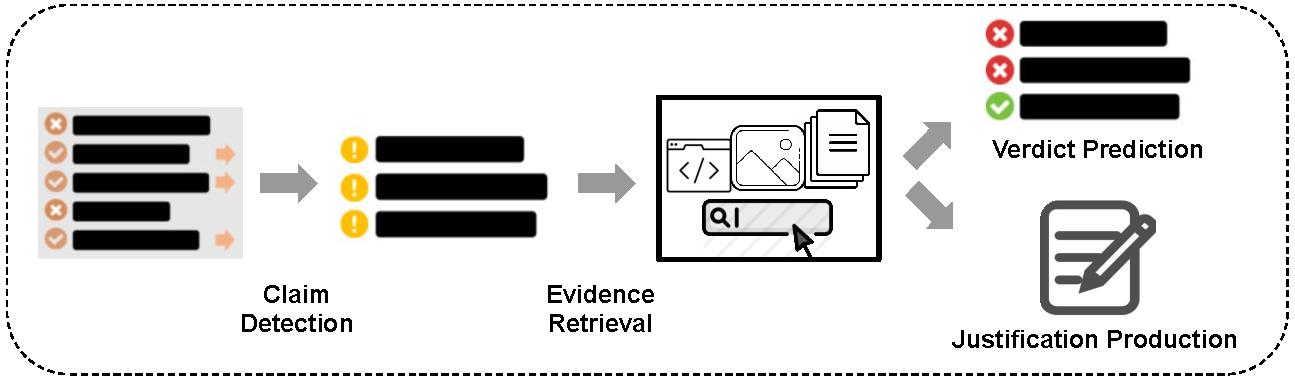
\includegraphics[width=14cm]{fig/framework.pdf}
    \caption{Automated fact-checking pipeline, reprinted from~\cite{guo-etal-2022-survey}}
    \label{fig:framework}
\end{figure}

Despite the existence of end-to-end fact-checking services, such as \url{politifact.org} or \url{demagog.cz}, the human-powered approach shows weaknesses in its scalability. By design, the process of finding an exhaustive set of evidence that decides the claim veracity is much slower than that of generating false or misguiding claims. Therefore, efforts have been made to move part of the load to a computer program that can run without supervision.

The common research goal is a fact verification tool that would, given a claim, semantically search provided knowledge base (stored for example as a \textit{corpus} of some natural language), propose a set of evidence (e. g. $k$ semantically nearest paragraphs of the corpus) and suggest the final verdict (Figure \ref{fig:pipeline}). This would reduce the fact-checker's workload to mere adjustments of the proposed result and correction of mistakes on the computer side. 

The goal of the ongoing efforts of {\textsf{FactCheck}} team at {\textsf{AIC CTU}}, as addressed in the works of~\cite{rypar,dedkova} and~\cite{gazo} is to explore the state-of-the-art methods used for fact verification in other languages, and propose a strong baseline system for such a task in Czech.


\section{A word on the Transformers}
\label{sec:transformers}
For the past six years, the state-of-the-art solution for nearly every Natural Language Processing task is based on the concept of \textit{transformer networks} or, simply, \textit{Transformers}. This has been a major breakthrough in the field by~\cite{vaswani}, giving birth to the famous models such as \textsf{Google}'s \textsf{BERT}~\cite{bert} and its descendants, or the \textsf{OpenAI}'s \textsf{GPT-3}~\cite{gpt3}.

In our proposed methods, we use Transformers in every step of the fact verification pipeline. Therefore, we would like to introduce this concept to our reader to begin with. 

Transformer is a neural model for \textit{sequence-to-sequence} tasks, which, similarly e.g. to the \textit{LSTM-Networks}~\cite{lstm}, uses the Encoder--Decoder architecture. Its main point is that of using solely the \textit{self-attention} mechanism to represent its input and output, instead of any sequence-aligned recurrence~\cite{vaswani}.

In essence, the \textit{self-attention} (also known as the \textit{intra-attention}) transforms every input vector to a weighted sum of the vectors in its neighbourhood, weighted by their \textit{relatedness} to the input. One could illustrate this on the \textit{euphony} in music, where every tone of a song relates to all of the precedent ones, to some more than to the others.

The full Transformer architecture is depicted in Figure~\ref{fig:transformer}.
%--- FIG: UTF forms
\begin{figure}
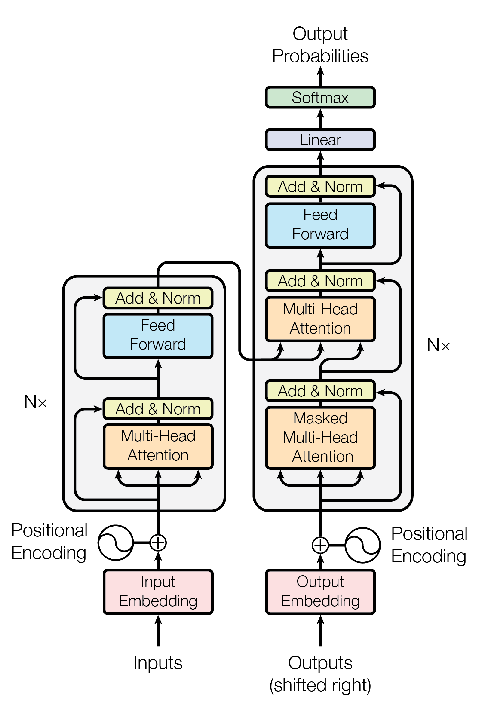
\includegraphics[width=9cm]{fig/transformer.pdf}
\caption{Transformer model architecture, reprinted from~\cite{vaswani}}
\label{fig:transformer}
\end{figure}
%--- /FIG



\section{Dissertation minimum study outline}
 
\begin{itemize}
\item {\techbf{Chapter~\ref{chap:intro}}} introduces the dissertation topic, motivates the research sets up our challenges for the future research 

\item {\techbf{Chapter~\ref{chap:sota}}} examines the most relevant research in the field and tries to highlight the recent paradigm shift from models trained for a single task to a single large models that perform well in everything

\item {\techbf{Chapter~\ref{chap:contribution}}} explains our current contributions to the field of automated fact-checking and NLP in Chech

\item {\techbf{Chapter~\ref{chap:plan}}} describes our plan for the dissertation and justifies the directions we are taking

\item Finally, {\techbf{Chapter~\ref{chap:conclusion}}} concludes the study with a wrapup of its findings

\end{itemize}


%%!TEX ROOT=../ctutest.tex
% UZAVŘENO! ÚPRAVY JEN ŽIVOTNĚ NUTNÉ NEBO VE ZBYLÉM ČASE

\chapter{Data Collection}
\label{chap:collection}
In Chapter~\ref{chap:intro}, we have introduced the framework of automated fact-checking. In order to construct an automated fact verifier, we first need methods of collecting the samples of Czech textual claims and their respective annotations within a fixed knowledge base.

These will allow us to assess the strength of the fact verifier in terms of compliance with human output for the same task. Furthermore, a dataset of sufficient size could be used to train statistical models.


\section{Related work}
As of May 2021, we have reviewed the following most notable papers and projects in the field, so as to provide proofs of concept and strong baselines..
\begin{itemize}
    \item {\techbf{Demagog dataset}}~\cite{hercig-lenc:2019:RANLP} -- dataset of verified textual claims in low-resource Slavic languages (9082 in Czech, 2835 in Polish, 12554 in Slovak), including their metadata s. a. the speaker's name and political affiliation.
    
    We have reviewed the Demagog dataset and deemed it not suitable for our purposes, as it does not operate under an enclosed knowledge base and rather justifies the veracity labeling through justification in natural language, often providing links from social networks, government operated webpages, etc.
    
    Even though the metadata could be used for statistical analyses, the loose structure of the data does not allow its straightforward use for the purpose of training/evaluation of NLP models.
    \item {\techbf{FEVER dataset}}~\cite{fever} -- \"{a large-scale dataset for Fact Extraction and VERification} -- dataset of 185,445 claims and their veracity labels from $\{\texttt{SUPPORTS},\texttt{REFUTES},\texttt{NOT ENOUGH INFO}\}$. Each label (except \texttt{NEI}s) is accompanied by a set of all\footnote{While this is assumed to be true by the \textsf{FEVER} benchmark, there are, in fact, valid evidence sets missing, due to the time constraints for the annotation task. In~\cite{fever}, 1\% annotations were re-annotated by \textit{super-annotators} tasked to find every possible evidence set without a time constraint, which has shown the precision/recall of the regular annotations to be 95.42\% and 72.36\%, respectively.} minimum evidence sets that can be used to infer the labelling. 
    
    It was extracted by 50 human annotators from approximately 50,000 popular \textsf{Wikipedia} article abstracts\footnote{The introductory section (i. e. the first paragraph) of \textsf{Wikipedia} article, one before the table of contents.} and fact-verified against every abstract in the full June 2017 \textsf{Wikipedia} dump.
    
    This is the most commonly used dataset used for validation of fact verification pipelines to date, and has been used as a benchmark in shared tasks~\cite{fever1,fever2adversarial} that inspired the publication of number of well-performing verifiers of English claims~\cite{papelo,athene,nie2019combining}.
    
    It was collected using a \textsf{Flask} app called the \textsf{FEVER Annotations Platform}, which has been partly open-sourced\footnote{\url{https://github.com/awslabs/fever}} and thoroughly described in~\cite{fever}.
    \item {\techbf{Danish fact verification datasets}}~\cite{danish} -- an effort to build an end-to-end fact verifier for the low-resource language of Danish, using the strategies employed by the submissions of the \textsf{FEVER} shared task~\cite{fever1} and \textsf{multilingual BERT}~\cite{devlin2019bert} for the Document Retrieval task.
    
    Binau and Schulte have handcrafted a dataset of 3,395 textual claims and their labels, along with evidence from the Danish \textsf{Wikipedia}, publishing an open source Command-line interface\footnote{\url{https://github.com/HenriSchulte/Danish-Fact-Verification}} for this task.
    
    They have also localized the large-scale \textsf{FEVER} dataset to Danish using the \textsf{Microsoft Translator Text API} and concluded separate experiments on the translated \textsf{FEVER DA} dataset.
\end{itemize}
We have not found an appropriate dataset for the NLP tasks we pursue, which is a common problem of a the non-international languages, such as Czech. We say that Czech is a \textit{low-resource} language, which, in NLP, signifies the need of adopting the methods and -- where possible -- the local versions of the corpora used for the tasks on foreign languages.

In order to train a verifier of our own for Czech (and for a whole different domain of the \textsf{ČTK} journal), we have attempted to repurpose the existing annotations of the \textsf{FEVER} dataset, as well as the annotation practices of both~\cite{fever} and~\cite{danish} where applicable.

The subsequent chapters introduce two of the resulting datasets that made it to production -- the {\techbf FEVER CS} and the {\techbf ČTK} dataset -- and the methods of their collection.

%-- TAB Fever, ctk
\begin{center}
\begin{table}[H]
\begin{ctucolortab}
\begin{tabular}{ c c c }
\textbf{Property} & {\techbf{}FEVER CS} & \techbf{ČTK} \\
\hline
\textbf{Obtained through} & Machine Translation & Annotation experiments\\
\textbf{Language style} & Encyclop\ae dic & Journalistic\\
\textbf{Retrieval unit} & Sentence & Paragraph\\
\textbf{Cross-references} & First level links & Knowledge scopes (\ref{sec:knowledge-scopes})\\
\textbf{Main focus} & Document retrieval & NLI (for the time being)\\
\textbf{Size} & 127,328 claims & 3,295 claims\\
\end{tabular}
\end{ctucolortab}
\caption{Comparison of \textsf{FEVER CS} and \textsf{ČTK} datasets}
\label{tab:notation-overview}
\end{table}
\end{center} 
%-- \TAB

%%!TEX ROOT=../ctutest.tex
% UZAVŘENO! ÚPRAVY JEN ŽIVOTNĚ NUTNÉ NEBO VE ZBYLÉM ČASE


\chapter{FEVER CS: a Dataset Localization}
\label{chap:fever_cs}
In Chapter~\ref{chap:collection}, we have examined the existing datasets for our task. In this chapter, we will attempt to extract a part of the correct fact verification examples they carry, and localize them into Czech. More specifically, we will be proposing localization methods for the greatest one -- the \textsf{FEVER} dataset.

Even though the localization process is prone to imperfections of all sorts, its resulting dataset will be of great use training the \textit{baseline} models, as well as \textit{pre-training} the finer models in the later stages of our work, when a native Czech dataset will be introduced for the \textit{fine-tuning}.
\section{FEVER format}
Before we start to extract the Czech $(claim,evidence)$ pairs, let us examine the format of the \textsf{FEVER} datapoints.

\begin{figure}[H]
\begin{lstlisting}[language=json]
{
  "id": 36242,
  "verifiable": "VERIFIABLE",
  "label": "REFUTES",
  "claim": "Mud was made before Matthew McConaughey was born.",
  "evidence": [
    [
      [52443, 62408, "Mud_-LRB-2012_film-RRB-", 1],
      [52443, 62408, "Matthew_McConaughey", 0]
    ],
    [
      [52443, 62409, "Mud_-LRB-2012_film-RRB-", 0]
    ]
  ]
}
\end{lstlisting}
    \caption{Example \textsf{FEVER} \texttt{REFUTES} annotation with two possible evidence sets}
    \label{list:fever}
\end{figure}

\begin{itemize}
    \item Dataset is stored in \texttt{JSON} Lines (\texttt{JSONL}) format, each line features a data point like~\ref{list:fever} without the whitespace
    \item The verifiability is stored in attribute $\texttt{verifiable}\in\{\texttt{VERIFIABLE},\texttt{NOT VERIFIABLE}\}$, veracity is stored using $\texttt{label}\in\{\texttt{SUPPORTS},\texttt{REFUTES},\texttt{NOT ENOUGH INFO}\}$ 
    \item \texttt{evidence} is a set of all possible \textit{evidence sets}, any of these sets \textit{alone} suffices to refute the \texttt{claim}
    \item Every such an \textit{evidence set} is structured as a conjunction of \textsf{Wikipedia} sentences in format: \texttt{[annotation\_id, evidence\_id, article\_wikiid, sentence\_index]}
    
\end{itemize}

\noindent To illustrate the correct interpretation of data from the example~\ref{list:fever}, there are two possible counterproofs for the claim \"{\textit{Mud was made before Matthew McConaughey was born.}}:

\begin{figure}[H]
    \centering

    \textit{Evidence set \#1:}
    \begin{ctucolortab}
    
    \fbox{\begin{minipage}{0.9\textwidth}
       \begin{hangparas}{2em}{1}
            \textbf{[Mud (film)]} Mud is a 2012 American coming-of-age drama film written and directed by Jeff Nichols.
            
            \textbf{[Matthew McConaughey]} Matthew David McConaughey (born November 4, 1969) is an American actor.
            
        \end{hangparas}
    \end{minipage}}
    \end{ctucolortab}

    ~
    
    \textit{Evidence set \#2:}
    
    \begin{ctucolortab}
    \fbox{\begin{minipage}{0.9\textwidth}
       \begin{hangparas}{2em}{1}
            \textbf{[Mud (film)]} The film stars Matthew McConaughey, Tye Sheridan, Jacob Lofland, Sam Shepard, and Reese Witherspoon.
        \end{hangparas}
    \end{minipage}}
    \end{ctucolortab}
    \caption{Evidence from data point~\ref{list:fever}}    
    \label{fig:evidence}
\end{figure}

\section{Localizing the FEVER}
\label{sec:fevercs}
Before we introduce the single steps, let us design a simple scheme for localizing it into an arbitrary language exploiting the ties between \textsf{FEVER} and \textsf{Wikipedia}:

Starting from the \textsf{FEVER}~\cite{fever} dataset:
\begin{enumerate}
    \item Merge the \textsf{FEVER} \textsf{train} and \textsf{dev} datasets into a joint dataset \textsf{fever\_en}
    \item Using \textsf{MediaWiki API}, map every \textsf{Wikipedia} article used in \textsf{fever\_en} evidences to its target localization, if none found, remove every \textit{evidence set} that contains it to create the \textsf{fever\_lang} -- in our case, the \textsf{fever\_cs} (Section~\ref{sec:fever-loss})
    \item Remove all \texttt{SUPPORTS} and \texttt{REFUTES} data points with empty evidence from \textsf{fever\_lang} 
        \item Download the current \textsf{Wikipedia} dump in the target language, parse it into a \textit{knowledge base} -- plain text corpus keyed by article name (Section~\ref{sec:wikidump})
    \item Localize every claim using the Machine Translation (Section \ref{sub:mach})
    \item Normalize every string value in \textsf{fever\_lang}, as well as the knowledge base, using the same Unicode normal form (Section~\ref{sub:canonical})
    \item Sample around $0.05\cdot|\textsf{fever\_lang}|$\footnote{This split size is proportional to that of \textsf{FEVER EN} -- it balances the labels to punish bias and favours the \textsf{train} size, due to the data-heavy nature of the task} annotations for each label using a fixed \textit{random seed}\footnote{This ensures the reproducibility}, store them as \textsf{dev}. Repeat for \textsf{test}.
    \item Store the rest of labels as \textsf{train}
\end{enumerate}

This scheme has notable weaknesses. Firstly, the evidence sets are not guaranteed to be exhaustive -- no human annotations in the target language were made to detect whether there are new ways of verifying the claims using the target version of \textsf{Wikipedia}. Furthermore, an unknown number of evidence has lost its validity, as the given \textsf{Wikipedia} localization lacks the specific information needed to conclude the fact-checking verdict.

With all of the dataset's flaws listed above to keep in mind, it is an exciting starting point, appropriate for training and validating both the early Document Retrieval and Natural Language Inference models. Therefore, we argue, it is a fruitful experimental dataset for both fields of our research.

Now, let us reinforce on the non-trivial points from the scheme above, specifically for our Czech instance.
\subsection{Czech Wikipedia (June 2020) corpus}
\label{sec:wikidump}
As an experimental \textit{knowledge base}, we are providing the \textsf{CS June 2020 Wikipedia dump} parsed into a plain text corpus using the \textsf{WikiExtractor} and structured into a \textsf{FEVER-}like knowledge base, i.e., a \textsf{SQLite} single-table\footnote{The table name is \db{Document}} database, providing every article \textit{abstract} from the \textsf{CSWiki} dump, structured as its \texttt{id}, \texttt{text} and its \texttt{sentences}-split, computed using the \textsf{Punkt}~\cite{punkt} sentence tokenizer. 

The resulting knowledge base can be downloaded from our webpage\footnote{\url{http://bertik.net/cswiki}} and the tools for its extraction are open-sourced in the section~\ref{sec:fever_result}.

\subsection{Localization data loss}
\label{sec:fever-loss}
For every article, \textsf{Wikipedia} provides a set of links to the same article in different foreign languages. This feature is powered by the \textsf{MediaWiki} database and can be accessed programatically through the \textsf{MediaWiki API}~\cite{mediawiki}. 

In the early stage of development, we have written the ad--hoc \textsf{localize\_dataset}\footnote{\url{https://github.com/heruberuto/fact-checking/blob/master/localize_dataset.py}} \textsf{Python} module to exploit this feature. Its outputs for the \texttt{cs} target language (measuring the \textit{data loss} in the step 2. of~\ref{sec:fevercs}) are \textit{highly} encouraging:

\begin{lstlisting}
    Of 12633 articles: 6578 preserved, 6055 lost, of which 84 due to normalization
    Of 145449 data points, 112969 survived the localization (of which 35639 was not verifiable), 32480 didn't
\end{lstlisting}

That means the majority of \textsf{FEVER-}adjacent articles \textit{do} have their Czech translation, and, even more surprisingly, whole \textbf{78\%} of claims can be fully (dis-)proven in at least one way using only the Czech \textsf{Wiki}. That is, in an ideal world where the Czech abstracts are semantically equivalent to their English counterparts and no \texttt{NOT ENOUGH INFO} annotations are lost due to a piece of knowledge unique to \textsf{CSWiki}.

Still, this is most often the case for the points we examined, and even though the original sentence indices from~\ref{list:fever} can not be trusted, the \texttt{wikiid} typically can. The \textit{precision/recall} (\ref{sec:recall}) metrics are yet to be done using human annotations, however, the empirical intuition would be that \textit{recall} took most of the damage (\textit{evidence sets} \"{forgotten} by our dataset).
\subsection{Tested Approaches for English-Czech Machine Translation}
\label{sub:mach}
As the Machine Translation model evaluation is a complex field of its own, and as the standard metrics such as BLEU~\cite{bleu} or SacreBLEU~\cite{sacrebleu} require a number of human-annotated reference translations, we do not possess the time to properly cover it in our research project. Thus, we are down to our own empirical observations of the translation quality. Our conclusions should be taken as such.

From the tools openly available online in a ready-to-use manner, we have examined the following (Table~\ref{fig:translators}):

\begin{enumerate}
    \item {\techbf{Google Cloud Translation API}}~\cite{google} was the platform we used to translate the first version of FEVER CS dataset, as it is convenient to use on a large set of data, and as it empirically yielded a \textit{comprehensible} translation for the majority of~claims.
    \item {\techbf{LINDAT Translation Service}}~\cite{lindat} uses {\textsf{CUBBITT}}~\cite{Popel2020} transformer model for machine translation and was released after its publication in \textsf{Nature} in September 2020. It performs on par with the top commercial-grade translators, however, it is published under a restrictive license for personal use.
    \item {\techbf{DeepL}}~\cite{deepl} released its English--Czech translation model for public use on March $17^{th}$ 2021. While we found out about it two weeks before the thesis submission deadline, we feature its outputs in the final dataset, as we have observed its translations to be superior both in the \textit{translation adequacy}\footnote{Preserving text meaning~\cite{Popel2020}} and the fluency of the resulting texts. We have found it to be very robust against homonyms\footnote{Words that can have different meanings (and therefore different Czech translations), which, typically, must be guessed from the context -- s. a. the \"{river \textit{bank}} and the \"{retail \textit{bank}}}, which is crucial for preserving the claim meaning and, therefore, the validity of transferred evidence.
\end{enumerate}

%---- TEXTBOX=TRANSLATORS
\begin{table}[H]
\begin{ctucolortab}
\begin{tabular}{ l r r | l }

    
    \textbf{Original claim} &\footnotesize{EN}& ~ & \textbf{\"{Harald V of Norway married a commoner.}}\\
    \hline
    \textbf{\textsf{Google Translate}} &\footnotesize{CS}&\footnotesize{April'20}& \"{Norská Harald V se oženila s občanem.}\\
    \textbf{\textsf{Google Translate}} &\footnotesize{CS}&\footnotesize{May'21}& \"{Harald V Norska si vzal prostého občana.}\\
    \textbf{\textsf{CUBBITT}} &\footnotesize{CS}&\footnotesize{May'21} & \"{Harald V. z Norska si vzal neurozenou ženu.}\\
    \textbf{\textsf{DeepL}} &\footnotesize{CS}&\footnotesize{May'21} & \"{Harald V. Norský se oženil s obyčejnou ženou.}\\
    \hhline{===|=}
    \textbf{Original claim} &\footnotesize{EN}& ~ & \textbf{\"{Indiana Jones has been portrayed by an actor.}}\\
    \hline
    \textbf{\textsf{Google Translate}} &\footnotesize{CS}&\footnotesize{April'20}& \"{Indiana Jones byl vylíčen hercem.}\\
    \textbf{\textsf{Google Translate}} &\footnotesize{CS}&\footnotesize{May'21}& \"{Indiana Jones byl zobrazen hercem.}\\
    \textbf{\textsf{CUBBITT}} &\footnotesize{CS}&\footnotesize{May'21} & \"{Indiana Jonese ztvárnil herec.}\\
    \textbf{\textsf{DeepL}} &\footnotesize{CS}&\footnotesize{May'21} & \"{Indiana Jones byl ztvárněn hercem.}\\
    \hhline{===|=}
    \textbf{Original claim} &\footnotesize{EN}& ~ & \textbf{\"{Manchester by the Sea has grossed money.}}\\
    \hline
    \textbf{\textsf{Google Translate}} &\footnotesize{CS}&\footnotesize{April'20}& \"{Manchester u moře rozdal peníze.}\\
    \textbf{\textsf{Google Translate}} &\footnotesize{CS}&\footnotesize{May'21}& \"{Manchester by the Sea vydělal peníze.}\\
    \textbf{\textsf{CUBBITT}} &\footnotesize{CS}&\footnotesize{May'21} & \"{Manchester by the Sea utržil peníze.
}\\
    \textbf{\textsf{DeepL}} &\footnotesize{CS}&\footnotesize{May'21} & \"{Film Manchester by the Sea vydělal peníze.}\\
\end{tabular}
\end{ctucolortab}
\caption[Machine Translator comparison using \textsf{FEVER} claims]{Machine Translator comparison using \textsf{FEVER} claims. Examples were cherry-picked to highlight the observed differences between translators.}
    \label{fig:translators}
\end{table}

%---- /TEXTBOX

\subsection{Unicode Normalization}
\label{sub:canonical}
 In the Unicode paradigm, the same diacritized character can be stored using several different representations~\cite{unicode}. To allow straightforward byte-wise comparisons on the low level (s. a. TF-IDF search, neural networks, \dots), one should eliminate this property using one of the \textit{Unicode normal forms}:
 
\begin{enumerate}
    \item {\techbf{NFD}} -- \textit{Normalization Form Canonical Decomposition} -- fully expands out the character (see Figure~\ref{fig:unicode}). Is faster to compute, but ultimately takes more space. Theoretically, it could be used to exploit the property of Czech, that the words that have similar undiacritized representations tend to be semantically close (e. g. \"{býti} and \"{bytí} share 4 bytes rather than 2 in NFD)
    \item {\techbf{NFC}} -- \textit{Normalization Form Canonical Composition} -- runs the NFD algorithm and then combines the characters where possible -- it runs longer, but the resulting strings take up less space
\end{enumerate}

%--- FIG: UTF forms
\begin{figure}[H]
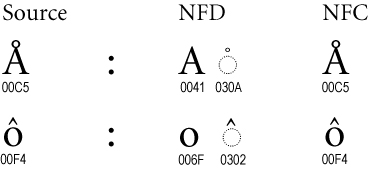
\includegraphics[width=6cm]{fig/UAX15-NormFig4.jpg}
\caption{Unicode normal forms, reprinted from~\cite{unicode}}
\label{fig:unicode}
\end{figure}
%--- /FIG

\subsection{Document leakage}
\label{sec:leakage}
An interesting and possibly malicious property of our dataset is a large \textit{document leakage} due to the simplistic splitting strategy defined in \ref{sec:fevercs} step 9.

Simply put, the \textsf{train} and \textsf{test} splits may contain claims related to the same evidence-set document. However, this was neither addressed by~\cite{fever}, as we have found \textbf{11,165} out of their \textbf{13,332} \textsf{dev}\footnote{Only the \texttt{SUPPORTS} and \texttt{REFUTES} annotations are considered in our measure, as the \texttt{NEI}s do not carry any evidence to compare against.}  annotations sharing an evidence-set document with some \textsf{train} claim. 

A further research is needed to answer whether this is a problem and what are the optimal strategies to punish model \textit{overfitting} while still optimizing for a broad topic coverage, proportional to the number of  leakage-prone documents.

\section{Resulting Dataset}

\label{sec:fever_result}
\begin{table}[H]
\begin{ctucolortab}
\begin{tabular}{ l | l l l || l l l  }
&  {\techbf{{FEVER CS}}} & & & {\techbf{{FEVER EN}}}&&\\
{} & {\texttt{SUPPORTS}} & \texttt{REFUTES}  & \texttt{NEI} & {\texttt{SUPPORTS}} & \texttt{REFUTES}  & \texttt{NEI}\\ 
\hline
{\tech train} & 53,542 & 18,149 & 35,639 & 80,035 &29,775& 35,639
\\
{\tech dev} & 3,333 & 3,333 & 3,333 & 6,666 & 6,666 & 6,666\\
{\tech test} & 3,333 & 3,333 & 3,333& 6,666 & 6,666 & 6,666\\
\end{tabular}
\end{ctucolortab}
\caption{Label distribution in \textsf{FEVER CS} dataset as oposed to the \textsf{FEVER EN}}
\label{tab:fevercs-overview}
\end{table}


In Table~\ref{tab:fevercs-overview} we show the label distribution in our dataset, is roughly proportional to that in \textsf{FEVER EN}. Inspired by the~\cite{fever} paper that only uses a \textsf{dev}, \textsf{test} of 3,333 claims per annotation to establish the baseline models, we have opted the same split size. This decision was experimental and should be further challenged in the future. 

Following the scheme described in~\ref{sec:fevercs}, we have released its open source implementations\footnote{\url{https://github.com/aic-factcheck/fever-cs-dataset}}~\footnote{\url{https://github.com/heruberuto/fact-checking/}} for an arbitrary language, and a set of ready-made \textsf{train}, \textsf{test} and \textsf{dev} data\footnote{\url{http://bertik.net/fever-cs}} in its most recent version Machine-Translated by \textsf{DeepL}. Both the data and the implementations are being published under the \textsf{CC BY-SA 3.0} license.

%%!TEX ROOT=../ctutest.tex

\chapter{ČTK Dataset Collection}
\label{chap:ctk}
In Chapter~\ref{chap:fever_cs}, we have acquired the initial fact-checking dataset in Czech via localizing that of~\cite{fever}. The localized dataset relies on the \textsf{Wikipedia} dump as its knowledge base.

As the \textsf{Wikipedia} does not call itself a reliable source for a multitude of reasons~\cite{wiki:reliable}, a further research is desirable on how to transfer the fact verification practice learned on \textsf{FEVER} to a whole other knowledge base.

This raises a variety of interesting challenges, in particular: how to transition away from the encyclop\ae{}dic style~\cite{wiki:style} of written language? Could one transfer the fact-checking rules learned on such a strictly formatted corpus to, say, an archive of {news reports}, with all of its pitfalls, such as the \textit{temporal reasoning}\footnote{Typical case would be a journal archive containing two mutually exclusive \textit{ground truths} different in their timestamps, s. a. \"{Summer 2018 was the warmest} and \"{Summer 2019 was the warmest}}?

\section{Academic Cooperations}
As a part of the project \textit{\"{Transformation of Ethical Aspects With the Advent of Artificial Intelligence Journalism}} funded by the \textsf{Technology Agency of the Czech Republic} (\textsf{TAČR}), we have been given an opportunity to work with Václav Moravec from the \textsf{Faculty of Social Sciences}, \textsf{Charles University} (\textsf{FSS}), and the students of his courses in \textit{AI Journalism}.

Furthermore, we have been granted access to the full archive of \textsf{Czech News Agency} (\textsf{ČTK}), that, by the time of creating a snapshot, contained a total of 15,032,152 news reports released between $1^{st}$ January 2000 and $6^{th}$~March~2019\footnote{Efforts are being made to re-insantiate the following data collection experiments on an extended version of the archive, up to December 2020, so as to cover the topic of COVID-19 pandemic. These were, however, postponed subsequent to this thesis, in order to maintain its data consistency.}, which we have reduced to the size of 11,134,727 reports by removing the sport results and daily news summaries.

Thanks to these cooperations, we have been offered to work with around 170 human annotators, mostly undergraduate and graduate students of \textsf{FSS}. During three \"{waves} of annotation, we have collected a total of 10,084 data points (3,293 original claims and their respective labels and evidence).

In this chapter, we would like to describe how we tailored our own annotation platform to the needs of our task and annotators, justify the design choices that we made, and summarize our experience of supervising three waves of human claim generation and labeling experiment.


\section{Requirements for the Annotation Platform}
\label{sec:requirements}
Before we unravel the solutions provided by our platform, let us first spend a section to establish the underlying problems. Even though we do not follow any strict procedure of the \textit{requirements modelling}~\cite{requirements}, we believe that what follows are the most important challenges our system should tackle and other researchers building such a tool might want to keep in mind:

\begin{enumerate}
    \item {\techbf FEVER-like annotation tasks} -- despite the corpus differences, we aim to follow the concept-proven task division from~\cite{fever}:
    \begin{enumerate}
        \item[\itembox{\textsf{WF1a}}] \textbf{Claim Extraction} provides annotator $A$ with a document $d$ from the \textsf{Wiki} corpus, $A$ outputs a simple factoid claim $c$ extracted from $d$ without using $A$'s own world knowledge
        \label{wf1a}
        \item [\itembox{\textsf{WF1b}}]\textbf{Claim Mutation}: feeds $c$ back to $A$, who outputs a set of mutations of $c$: \\
        $M^c=\{m^c_1,\dots m^c_n\}$ using $A$'s own world knowledge (\textit{negation},~\textit{generalization},~\dots).
        
        For the completeness, we reprint the Table~\ref{fig:mutations} that lists the allowed types of mutations.\label{wf1b}
        
        %--- FIG: UTF forms
\begin{table}[H]
\begin{ctucolortab}
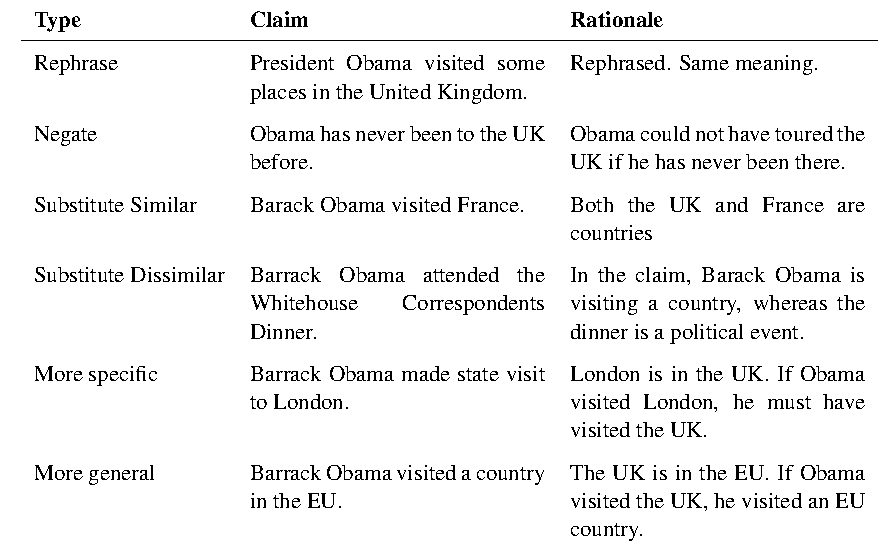
\includegraphics[width=12cm]{fig/mutations.pdf}
\caption[\textsf{FEVER Annotation Platform} mutation types]{\textsf{FEVER Annotation Platform} mutation types -- the examples mutate the claim \"{Barack Obama toured the UK} -- reprinted from~\cite{fever}}
\label{fig:mutations}
\end{ctucolortab}
\end{table}
%--- /FIG
        \item[\itembox{\textsf{WF2~}}] \textbf{Claim Labeling}: $A$ is given a sample of a mutated claim $m^c$, context that was given to extract $c$ in (a.) and is tasked to output sets of evidence $E^{m^c}_1,\dots,E^{m^c}_n$ along with the veracity label $g(E^{m^c}_i,m^c)$ which should be the same for each $i$. 
        \label{wf2}
        
        Apart from the context of $c$, $A$ can fulltext search the entire \textsf{Wikipedia} for evidence, however, $A$ operates under constrained time.
    \end{enumerate}
    
    \item {\techbf Paragraph-level documents} -- the \textsf{FEVER} shared task proposed a \textit{two-level} retrieval model: first, a set of \textit{documents}, i.e., \textsf{Wiki} abstracts is retrieved, then these are fed to the \textit{sentence retrieval} system which retrieves the evidence on the level of sentences.
    
    This simply does not work for us -- firstly, the sentences of a news report corpus are significantly less \textit{self-contained} than those of encyclop\ae{}dia abstract, not supporting the \textit{sentence}-level of granularity. Secondly, the articles tend to be overly long for the Document Retrieval task. 
    
    We argue that the best approach for our data is the \textit{paragraph-wise} splitting and a single level of retrieval, with an option of grouping a set of paragraphs by their source article. From this point we refer to the \textsf{ČTK} paragraphs also as to the \textit{documents}.
    
    \item {\techbf Source document sampling system} -- in~\cite{fever}, every claim was extracted from some sentence sampled from a \textsf{Wikipedia} abstract. With news report archive, this does not work well, as the majority of \textsf{ČTK} paragraphs does not contain an information eligible for fact-checking.
    \item {\techbf Limited knowledge oracle access} -- in \textsf{FEVER} \textbf{Claim Extraction} as well as in the annotation experiment of~\cite{danish}, the annotator was provided with a \textsf{Wikipedia} abstract and a \textit{dictionary} composed of the abstracts of articles \textit{linked} in it. This was important to ensure that the annotators only incorporate their full world knowledge in a restricted number of well defined tasks, and limit themselves to the facts (dis-)provable using the corpus in the rest.
    
    As the \textsf{ČTK} corpus does not follow any rules for internal linking, this will be a major challenge to reproduce. 
    \item {\techbf Annotator performance measures} -- completion of the annotation tasks is going to count towards the completion of the \textsf{FSS} course. Therefore, the annotator's identity needs to be stored within the system, and a set of reasonable goals must be proposed to track the completion of student's duties. 
    
    Reaching the goals should take under 3 hours on average, which matches the share of the annotation assignment on the \textsf{ECTS} study load of the \textsf{FSS} course~\cite{ects}.
    
    \item {\techbf Cross-annotator validation} -- to measure the validity of the annotations, as well as that of our novel platform, a claim should be labeled more than once on average.
    
    This will allow us to quantify the inter-annotator agreement, as well as it increases the overall number of evidence sets per claim. We do not consider the task of enumerating \textit{every} possible evidence set from the \textsf{ČTK} corpus feasible, as the news archives are not limited in the number of duplicate information they store. However, the more the better.
    
    \item {\techbf ČTK Archive access mediation} -- Due to the size of the \textsf{ČTK} archive (\char`~11M reports with metadata) and our space constraints that do not allow a very generous indexing, we need a caching system that only stores the articles necessary for annotating the claims that are currently in the system. This reduces the lookup time and increases the maximum traffic load.
\end{enumerate}

\section{FCheck Platform}
In Figure~\ref{fig:er}, we model the basic structures of data our system is working with and their relations using the standard entity--relationship diagram~\cite{10.1145/320434.320440}.

In contrast with the simplicity of the structured \textsf{JSONL} annotation format shown in the Figure~\ref{list:fever}, our data model is rather complex. Our aim here is to exploit the properties of relational database to find annotation ambiguities and easily compute the annotator performance measures through \textsf{SQL} \textit{aggregations}

In addition, we introduce the automatically updated \textsf{UNIX} timestamps \texttt{created\_at} and \texttt{updated\_at} to every entity from~\ref{fig:er}, to be able to reconstruct the annotation timeline, as well as to generate a dashboard of {live} visualisations of the performance and validity metrics, examples of which are the Figure~\ref{fig:crossannotations} and~\ref{fig:performance}.

\subsection{Entities and Their Relations}

Every annotator is to be identified through their respective \db{User} object, storing the neccessary credentials and signing every annotated data-point with their identifier. The data-points are divided into \db{Claim}s and \db{Label}s. Each \db{Claim} is either extracted from a \textsf{ČTK} \db{Paragraph}, linked as \texttt{paragraph}, or from a parent \db{Claim}, linked as \texttt{mutated\_from}.

\begin{figure}[H]

 \makebox[\textwidth][c]{{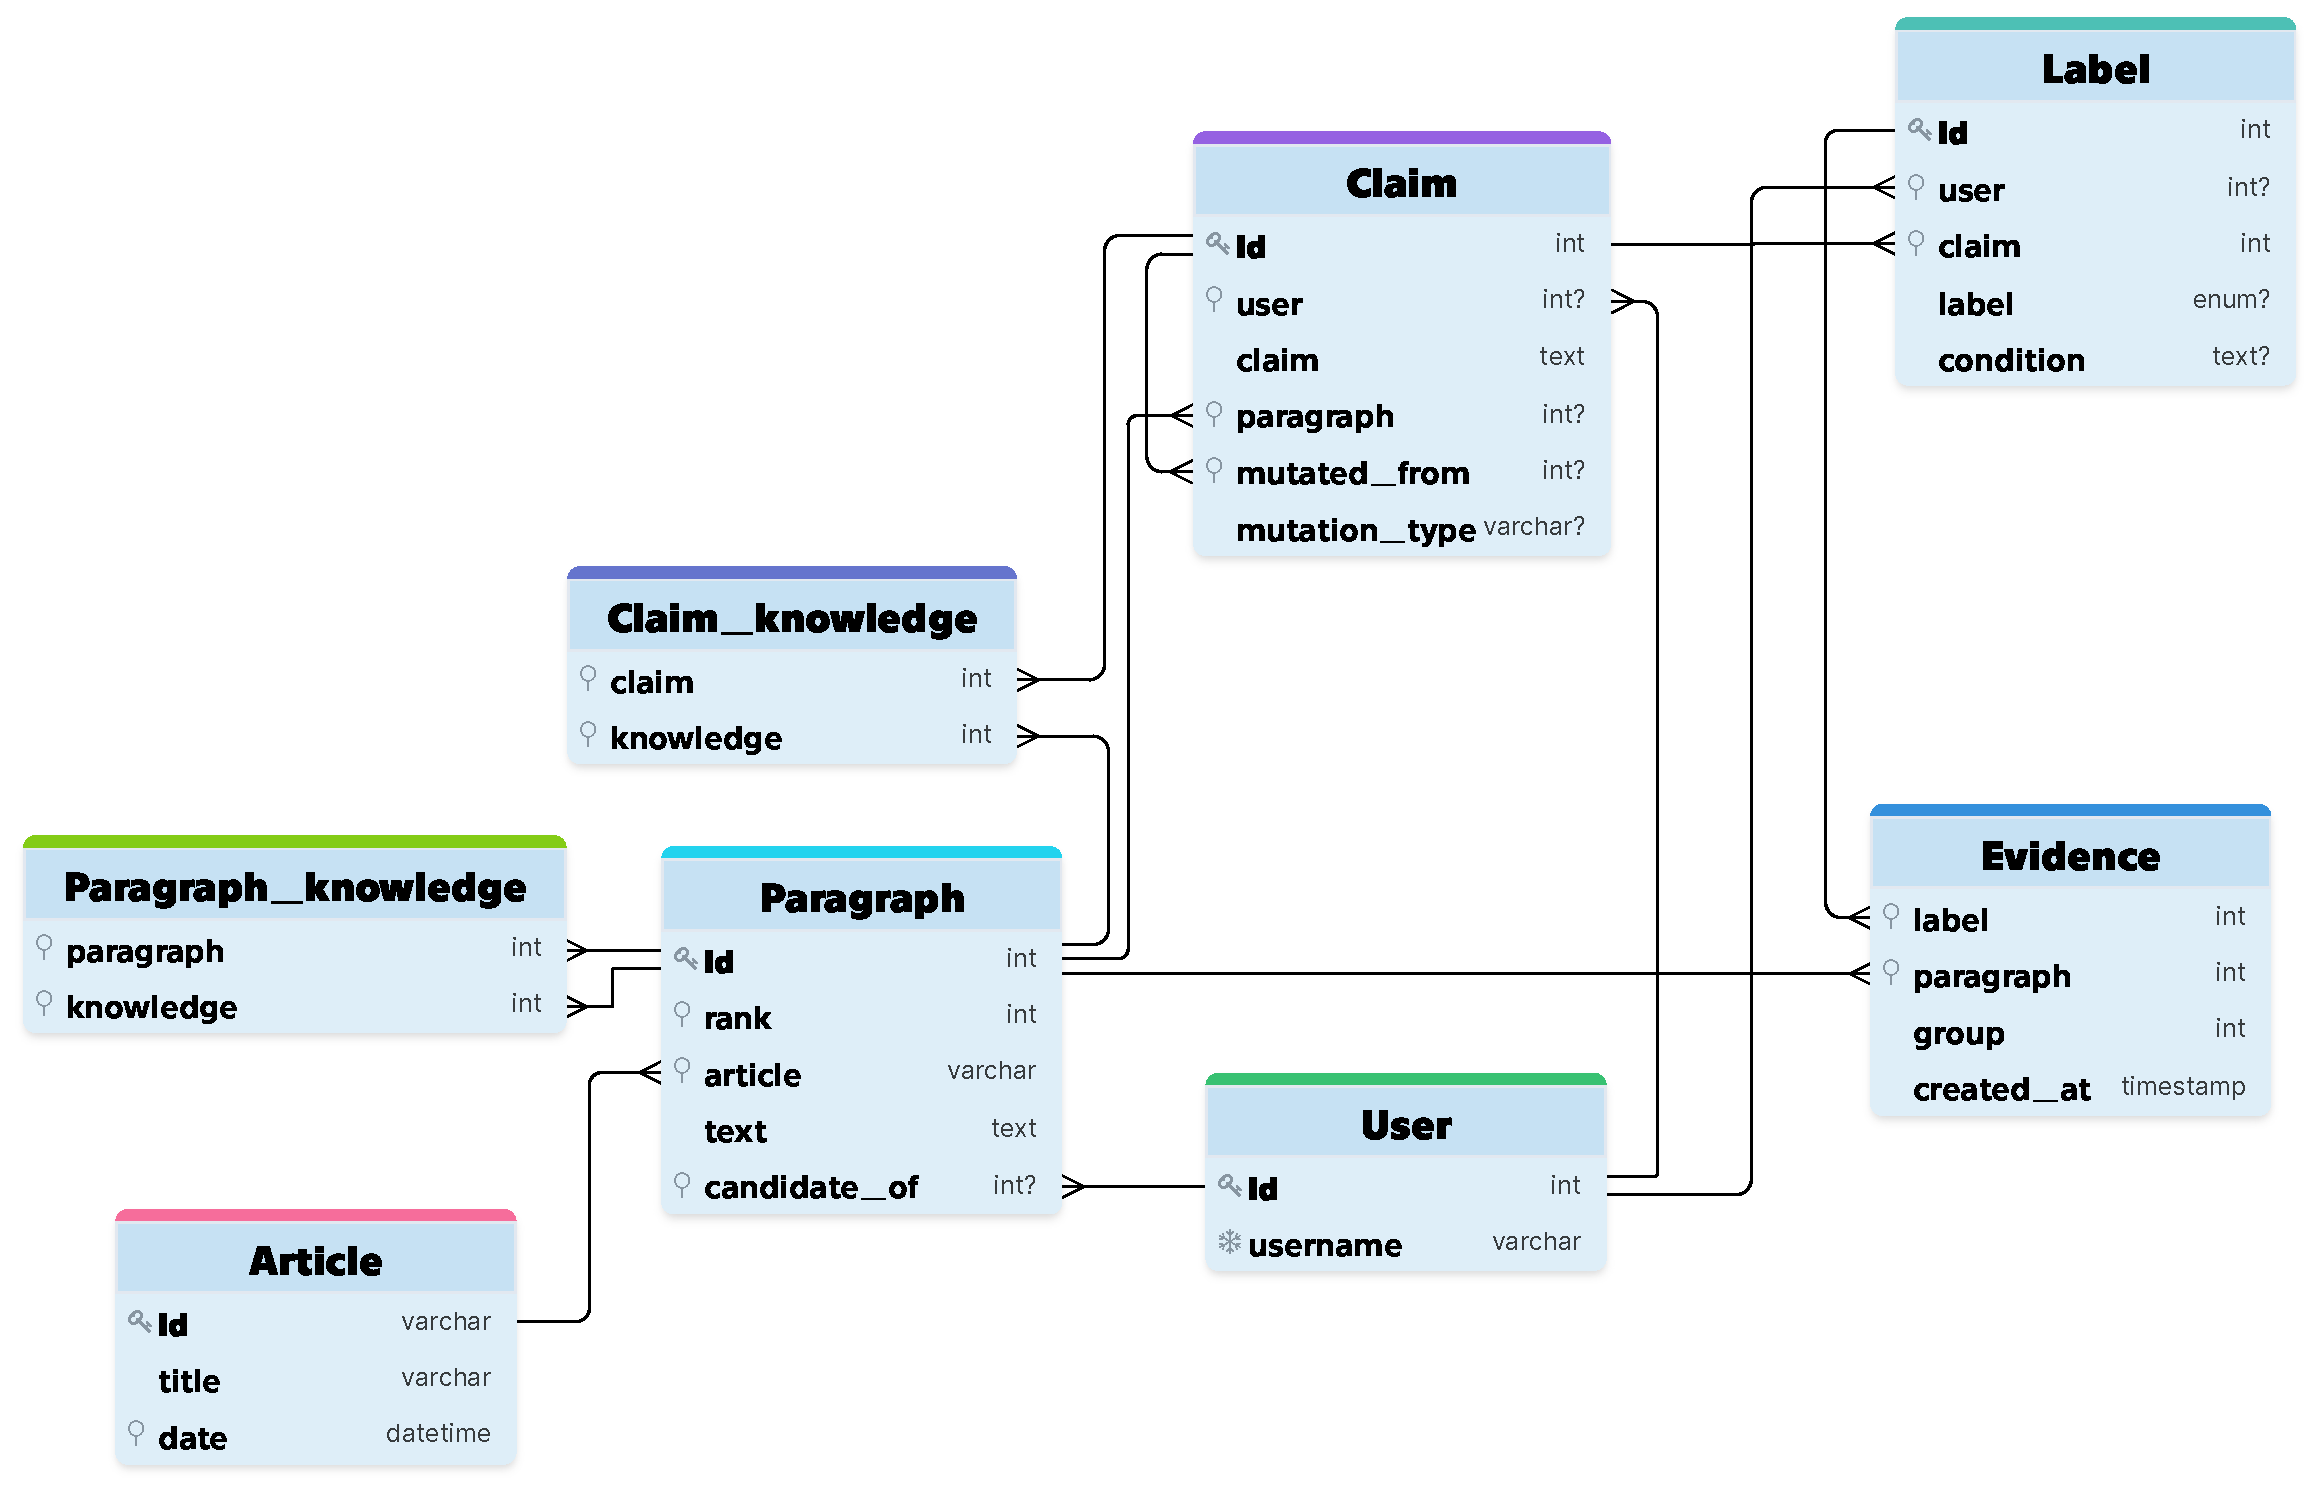
\includegraphics[width=18cm]{fig/er-diagram.pdf}}}

\caption{Entity--relationship diagram of the {\textsf{FCheck}} application drawn using \cite{drawsql}}
\label{fig:er}
\end{figure}%ER diagram

For the Claim Labeling and Claim Extraction tasks, user is to be given a restricted scope of knowledge. This knowledge can be described as a set of \db{Paragraph} objects, and is defined for a given \db{Claim} or \db{Paragraph} (\textit{many-to-many} relations \db{Paragraph\_knowledge} and \db{Claim\_knowledge}) -- we will define the \textit{knowledge scopes} in~\ref{sec:knowledge-scopes}.

The \db{Label} data-point is characterized by the \texttt{label} itself (\texttt{\textit{enum}} of \texttt{SUPPORTS},\texttt{REFUTES},\texttt{NOT ENOUGH INFO}) and its \db{Evidence} -- a set of \textit{evidence sets}. Each such evidence set consists of \db{Paragraph}s and is distinguished by a different ordinal number \texttt{group} stored alongside the \db{Evidence} relation. Therefore, a single \db{Label} can have multiple alternate sets of evidence, just as demonstrated in the Figure~\ref{list:fever}. 

Several complementary entities were hidden away for the simplicity of the~\ref{fig:er}, however, are not integral to the data model of our application -- for example the \textit{annotation stopwatch} data.

\subsection{Technology Stack}
Originally, we have planned to re-use the \textsf{Flask} annotation platform of~\cite{fever} with minor tweaks. Sadly, we were unable to fully recover the open source version\footnote{\url{https://github.com/awslabs/fever/tree/master/fever-annotations-platform}}, as there was static data of unknown structure missing for \textsf{Wiki} \textit{redirects}.

Even so, these efforts would have been rendered futile by the invention of \textit{knowledge scopes} that we will introduce in~\ref{sec:knowledge-scopes}.

Thus, we have embarked on the journey to build our very own annotation platform, heavily inspired by that of~\cite{fever}, using our preferred technologies:

\begin{enumerate}
    \item {\techbf PHP 7} will be running the annotation back-end, written using the {\techbf Yii2} framework, served by {\techbf Apache2} on {\techbf Debian} 
    \item {\techbf MySQL 8} is to be storing the entities from~\ref{fig:er} in form of the \textsf{SQL} tables
    \item {\techbf Python 3.7}, {\techbf PyTorch}, {\techbf Flask} and {\techbf SQLite3} provide an \textsf{API} for a direct {\textsf{ČTK}} data access, as well as to the neural networks and clustering required for semantic search
    \item {\techbf AJAX} will be used to asynchronize the \textsf{API} calls, so that a user can keep annotating on the \textsf{Apache} server while the computation-heavy tasks are being processed by \textsf{Flask}
\end{enumerate}
Despite the choice of technologies does not follow the most recent trends, we have decided for it because of its familiarity. As the annotation leadership and administration are tasks heavy on technical support and hotfixing, we favoured the tools we have several years of commercial experience with.


\subsection{Corpus Caching: Proxy Entities}
\label{sec:proxies}
The \db{Article} and \db{Paragraph} \textsf{db} entities from~\ref{fig:er} serve as a proxy for the slowly attainable entries of the full \textsf{ČTK} corpus which is stored separately and its paragraphs are copied to the \textsf{FCheck} database on demand.

The idea is that if we provide a background service that asynchronously precomputes which paragraphs of the full corpus are to be provided to an annotator for the given task and input data, we can simply copy them into a well-indexed smaller database integrated with the rest of the system through a relational database. 

Thus, we were able to scale down the amount of data hardwired to the interactive part of the platform from \char`~$10^8$ to the order of $10^4$ paragraphs, dramatically improving the lookup times while also obtaining a compact \textit{self-contained}  database that can be easily backed up and still contain all the corpus entries necessary for exporting the dataset.


\subsection{Knowledge Scopes}
\label{sec:knowledge-scopes}
\textit{In place of \textsf{Wikipedia} \textit{dictionaries} that were used used in \textsf{FEVER} annotation task, we propose the following framework for knowledge delimitation:}



We have used the \textsf{DrQA}~\cite{drqa} and \textsf{multilingual BERT}~\cite{devlin2019bert} models trained by~\cite{michal} during his summer \textsf{AIC} internship as our internal state-of-the-art for \textsf{FEVER CS} \textsf{wiki-}abstract retrieval. The model task was to output a set of $k$ semantically nearest paragraphs ($k$-NN) to the given string.

Where \textsf{DrQA} operates on a verbatim (\textit{term frequency–inverse document frequency}) basis, \textsf{mBERT} model calculates the paragraph \textit{embeddings} using a Transformer network pre-trained on \textsf{Wikipedia} and finetuned for the Czech Document Retrieval task.

To have the best of both worlds, we have used a simple \textsf{ČTK Archive Flask API}, implemented by~\cite{honzagit} as a \textit{façade} that receives a claim (or a paragraph identifier) through a \textsf{HTTP} request, and responds with a combination of the results of both of the aforementioned models.

\subsubsection{ČTK Archive Flask API}
Is a simple \textsf{HTTP API} we have co-authored with our supervisor Jan Drchal. It encapsulates the access to the \textsf{ČTK Archive} corpus via \textit{random sampling} and the \textit{Knowledge scope} enumeration, which follows:

In brief words, it makes multiple calls to the \textsf{DrQA}, fortifying the claim by a different pair of mentioned \textit{named entities} in each\footnote{E. g. the claim \"{Miloš Zeman visited Slovakia.} is augmented by an extra copy of the entity \"{Miloš Zeman}, and \"{Slovakia}, to boost their \textit{term frequency}.}, to obtain their highest-utility results for each NE pair. Then it picks the 4 documents with the \textit{overall} highest utility as the \texttt{search\_ner} result. The Named Entity Recognition is handled by the model of~\cite{strakova-etal-2019-neural}.

It then retrieves the 1024 top documents for the query using \textsf{mBERT}, and clusters their embeddings into 2 groups with $k$-means. Then, two closest representatives of the \textit{claim embedding} from every cluster are stored as the \texttt{search\_semantic}.

The flask ouputs both \texttt{search\_ner} and \texttt{search\_semantic}, i.e., a maximum of 8 documents per query, not to overwhelm the annotator. Furthermore, it makes sure that all the retrieved paragraphs have an older timestamp than the input. This outlines our solution for the \textit{temporal reasoning} issue. Simply put, to each claim, we assign a date of its formulation, and only verify it using the news reports published \textit{to that date}.

Using the example from the~\hyperref[chap:ctk]{chapter introduction}, the paragraph \"{Summer 2019 was the warmest} (say, published at Septamber $24^{th}$, 2019) will only be considered a \textit{ground truth} for claims with a timestamp $\geq \texttt{2019-09-24}$. For the completeness, later, in the task \tjednab{}, we assign each claim with the publication timestamp of its source paragraph.

\section{The Annotation Workflow}
In the previous sections, we have explained the technical challenges and their respective solutions. An equally important task is that of supervising a group of annotators new to this system and streamlining a sequence of tasks that both guides the annotators to the best use of their expertise in journalism and saturates the dataset.



\subsection{Revised Annotation Tasks}


To satisfy our requirements, we have adjusted the annotation tasks from Section~\ref{sec:requirements} in the following ways: 

\textit{For reader's convenience, we mostly use a simplified set of actors -- \textsf{Flask} is the \"{slow} back-end \textsf{API}, that operates above with the full \textsf{ČTK Archive} and models from~\ref{sec:knowledge-scopes}, \textsf{Apache} is a lighter web interface above the entities of~\ref{fig:er} accessible to $A$, $A$ is the annotator.}
\begin{enumerate}
        \item[\itembox{$\textsf{T}_{\textsf{0~}}$}] \textbf{Source Paragraph Preselection:} \textsf{Flask} samples a source article, \textsf{Apache} caches it (see~\ref{sec:proxies}). $A$ spends $~\leq 30$ seconds skimming the article and, finally, nominates a single paragraph $p$ to be used in $\textsf{T}_{\textsf{1a}}$. 
        
        $p$ must feature a \textit{self-contained} piece of verifiable information. If there is no such paragraph, $A$ skips to the next sample. 
        
        Otherwise, \textsf{Apache} stores the nomination and \textsf{Flask} enqueues the \textit{knowledge scope} computation for $p$. Once finished, result will be forwarded to \textsf{Apache}, which will cache the retrieved paragraphs and their respective articles and store them as $knowledge(p)$.
        
        
        \label{t0}
        \item[\itembox{$\textsf{T}_{\textsf{1a}}$}] \textbf{Claim Extraction:} \textsf{Apache} samples a nominated paragraph $p$, provides $A$ with $p$ and $knowledge(p)$. $A$ outputs a simple factoid claim $c$ extracted from $\{p\}\cup knowledge(p)$ without using $A$'s own world knowledge
        \label{t1a}
        \item [\itembox{$\textsf{T}_{\textsf{1b}}$}]\textbf{Claim Mutation}: \textsf{Apache} feeds $c$ back to $A$, who outputs a set of mutations of $c$: \\
        $M^c=\{m^c_1,\dots m^c_n\}$ using $A$'s own world knowledge (\textit{negation},~\textit{generalization},~\dots)\label{t1b}
        
        To catch up with the additional knowledge introduced by $A$, \textsf{Flask} enqueues the computation of $\{knowledge(m^c_1),\dots knowledge(m^c_n)\}$, and, once done, notifies \textsf{Apache} to store these, as well as to cache the incident paragraphs.
        \item[\itembox{$\textsf{T}_{\textsf{2a}}$}] \textbf{Own (Oracle) Claim Labeling}: \textsf{Apache} samples a fresh $m^c$ made by $A$, and provides its source paragraph $p$, its full original article, and a shuffled set of articles from $knowledge(m^c)\cup knowledge(p)$.
        
        $A$ spends $\leq 3$ minutes looking for the evidence sets  $E^{m^c}_1,\dots,E^{m^c}_n$ along with the veracity label $g(E^{m^c}_i,m^c)$. \textsf{Apache} saves them as an \textit{oracle annotation}.
        \label{t2a}
        
                \item[\itembox{$\textsf{T}_{\textsf{2b}}$}] \textbf{Others' Claim Labeling}: same as \tdvaa{} for $m^c$ made by \textit{other} annotator than $A$. Stored as \textit{regular annotation}.
        \label{t2b}
    
    \end{enumerate}

\subsection{Conditional annotations}
During our tests of the interface, a common problem with the annotation task \tdva{} using the \textsf{ČTK} corpus was that of \textit{assuming the knowledge}. Using the mutation types such as \textit{generalization}, one would often run into generating a claim containing a mutation not fully provable using a news archive.

For example, for a claim \"{Miloš Zeman did not visit an European country}, system~\ref{sec:knowledge-scopes} often retrieves relevant knowledge s. a. \"{Miloš Zeman visited Slovakia}. However, it barely ever retrieves the neccessary conclusive proof that \"{Slovakia is a European country}.

To address this issue, we are introducing the concept of \textit{conditional annotations}: if the annotator can not construct an exhaustive evidence set, but possesses knowledge that would \textit{conclude} the \textit{partial} set of evidence, he is asked to write it down in a form of \textit{textual claim} $c_{condition}$. Then, if any annotator could \texttt{SUPPORT} the $c_{condition}$ using a freshly computed $knowledge(c_{condition})$, it would also yield the paragraphs that would \textit{complete} the partial sets of the original evidence.

\label{sub:conditional}
\begin{figure}[H]

    \begin{ctucolortab}
    
    \fbox{\begin{minipage}{\textwidth}
        \textbf{Claim:} \"{The Killers performed in \textbf{the second day} of Rock for People 2007.}
        
        \textbf{Label: }\texttt{REFUTES}
        
        \textbf{Condition:} \"{The first and the second day of Rock for People had disjoint line-ups.}
    \end{minipage}}
    \end{ctucolortab}

    ~
    

    \textit{Evidence set \#1:}
    \begin{ctucolortab}
    
    \fbox{\begin{minipage}{\textwidth}
\begin{hangparas}{2em}{1}
            {\textbf{The first day of Rock for People culminated with the concert of The~Killers [July $4^{th}$ 2007]}} 
            
            \hspace{1.7em} Hradec Králové, 4th of July (ČTK) - Today, an hour before midnight at the Hradec Králové airport, American guitar band The Killers performed their concert, which was the climax of \textbf{the first day} of the festival. Above the mucisians' heads hanged a shining sign \"{Sam's Town}, which is the name of their second album that came out last year. The musicians came to introduce the songs from this album to the festival audience.
\end{hangparas}
    \end{minipage}}
    \end{ctucolortab}

    
    \caption[Example of a conditional label]{Example of a conditional label (translated from the \textsf{ČTK v2.1} dataset). See that if we are able to \texttt{SUPPORT} the \textbf{condition}, we can use the union of any of its evidence-sets together with the set \textit{\#1} to disprove the original claim. If not, the correct label is \texttt{NEI}.}
    \label{fig:conditional}
\end{figure}

\section{Web User Interface}
Finally, we are including a look into the client-side of the annotation platform we have presented to our annotators. 

In~\ref{sec:requirements}, we have estimated a maximum time of \textbf{3 hours} to complete the entire annotation workflow (\ref{fig:annotation}). Of these, we have dedicated the first \textbf{30 minutes} to a \textbf{video-tutorial}\footnote{\url{https://fcheck.fel.cvut.cz/site/tutorial} or \url{https://youtu.be/AcarF4Rxexc}}, which, despite its length, worked well\footnote{
After refining the tutorial and the supplementary lecture after the first wave of annotations, we have observed a significant decrease in the task procrastination (see Figure~\ref{fig:performance}), which may also have been caused by other factors. However, it had a good impact on the traffic spread, as well as on the quality of \tdva{} sampling (Figure~\ref{fig:crossannotations}).} in giving every annotator a full platform walkthrough and a hands-on example for every task.

Therefore, each student should spend only \textbf{2.5 hours} on our platform to reach all the annotation goals from Figure~\ref{fig:annotation}. This puts pressure on the design of the client-side, to be as easy to use as possible, while still supporting the sophisticated features, s. a. the \textit{conditional-} and \textit{multi-annotation}. In this chapter, we will show the web interface for the main tasks, and justify the design choices made.

To our readers, we also provide the link to the live\footnote{For as long as the \textsf{FEE CTU} keeps providing us with the computing power\dots} platform which can be found at \url{https://fcheck.fel.cvut.cz} and accessed by typing  \texttt{testuser} into the \"{\textsf{SIDOS} ID} field. Do not worry to play around, as all of the \texttt{testuser}'s annotations can be easily omitted from the exports.

\subsection{Claim Extraction}
We present our final \tjednaa{} interface in Figure~\ref{fig:annotation}. The layout is inspired by the work of~\cite{fever} and, by default, hides as much of the clutter away from the user as possible. Except for the article heading, timestamp and the source paragraph, all the information such as the \textit{knowledge base} is collapsed and only rendered on user's demand. 

During the first run, user is instructed to read through detailed {\btn{Instructions}} in a \textsf{Bootstrap} \textit{modal} window, that, for the rest of the time, stay hidden away again not to distract the annotator. Apart from these, we have only added a brief instruction to each the form field as a reminder.

Annotator reads the source article and, if it lacks a piece of information he wants to extract, looks for it in the expanded article or knowledge base entry. Extracted claims are to be typed into a \textsf{HTML} textarea and separated by the line break, which was the most intuitive method we experimented with. User is encouraged to \btn{Skip} any source paragraph that is hard to extract. 

Throughout the platform, we have ultimately decided not to display any \textit{stopwatch}-like interface not to stress out the user. However, there is a simple tracking \textsf{JavaScript} running in the background, storing time spent on each page. From this data, we have measured that, excluding the outliers ($\leq10s$, typically the \btn{Skip}ped annotations and $\geq 600s$, typically a browser tab left unattended), average time spent on this task is \textbf{2 minutes 16 seconds} and the median is \textbf{1 minute 16 seconds}.

After the first wave of annotation, we have augmented the interface with a triple of \textit{golden rules} to avoid repeating the most common mistakes. More on that in~\ref{sec:golden-rules}.



\subsection{Claim Mutation}
Follows the UI conventions set by the Claim Extraction. Mutation types follow those of the \textsf{FEVER Annotation Platform} (Table~\ref{fig:mutations}) and are distinguished by loud colors, to avoid mismatches. The mutation types will be a topic for further innovations in future, as our annotation experiments did not yield a label-balanced dataset. 

Excluding the outliers, the overall average time spent generating a batch of mutations was \textbf{3m 35s} (median \textbf{3m 15s}) with an average of \textbf{3.98} mutations generated per claim.

\pagebreak
\begin{figure}[H]
\thispagestyle{empty}
\vspace{-1.5cm}
\makebox[\textwidth][c]{{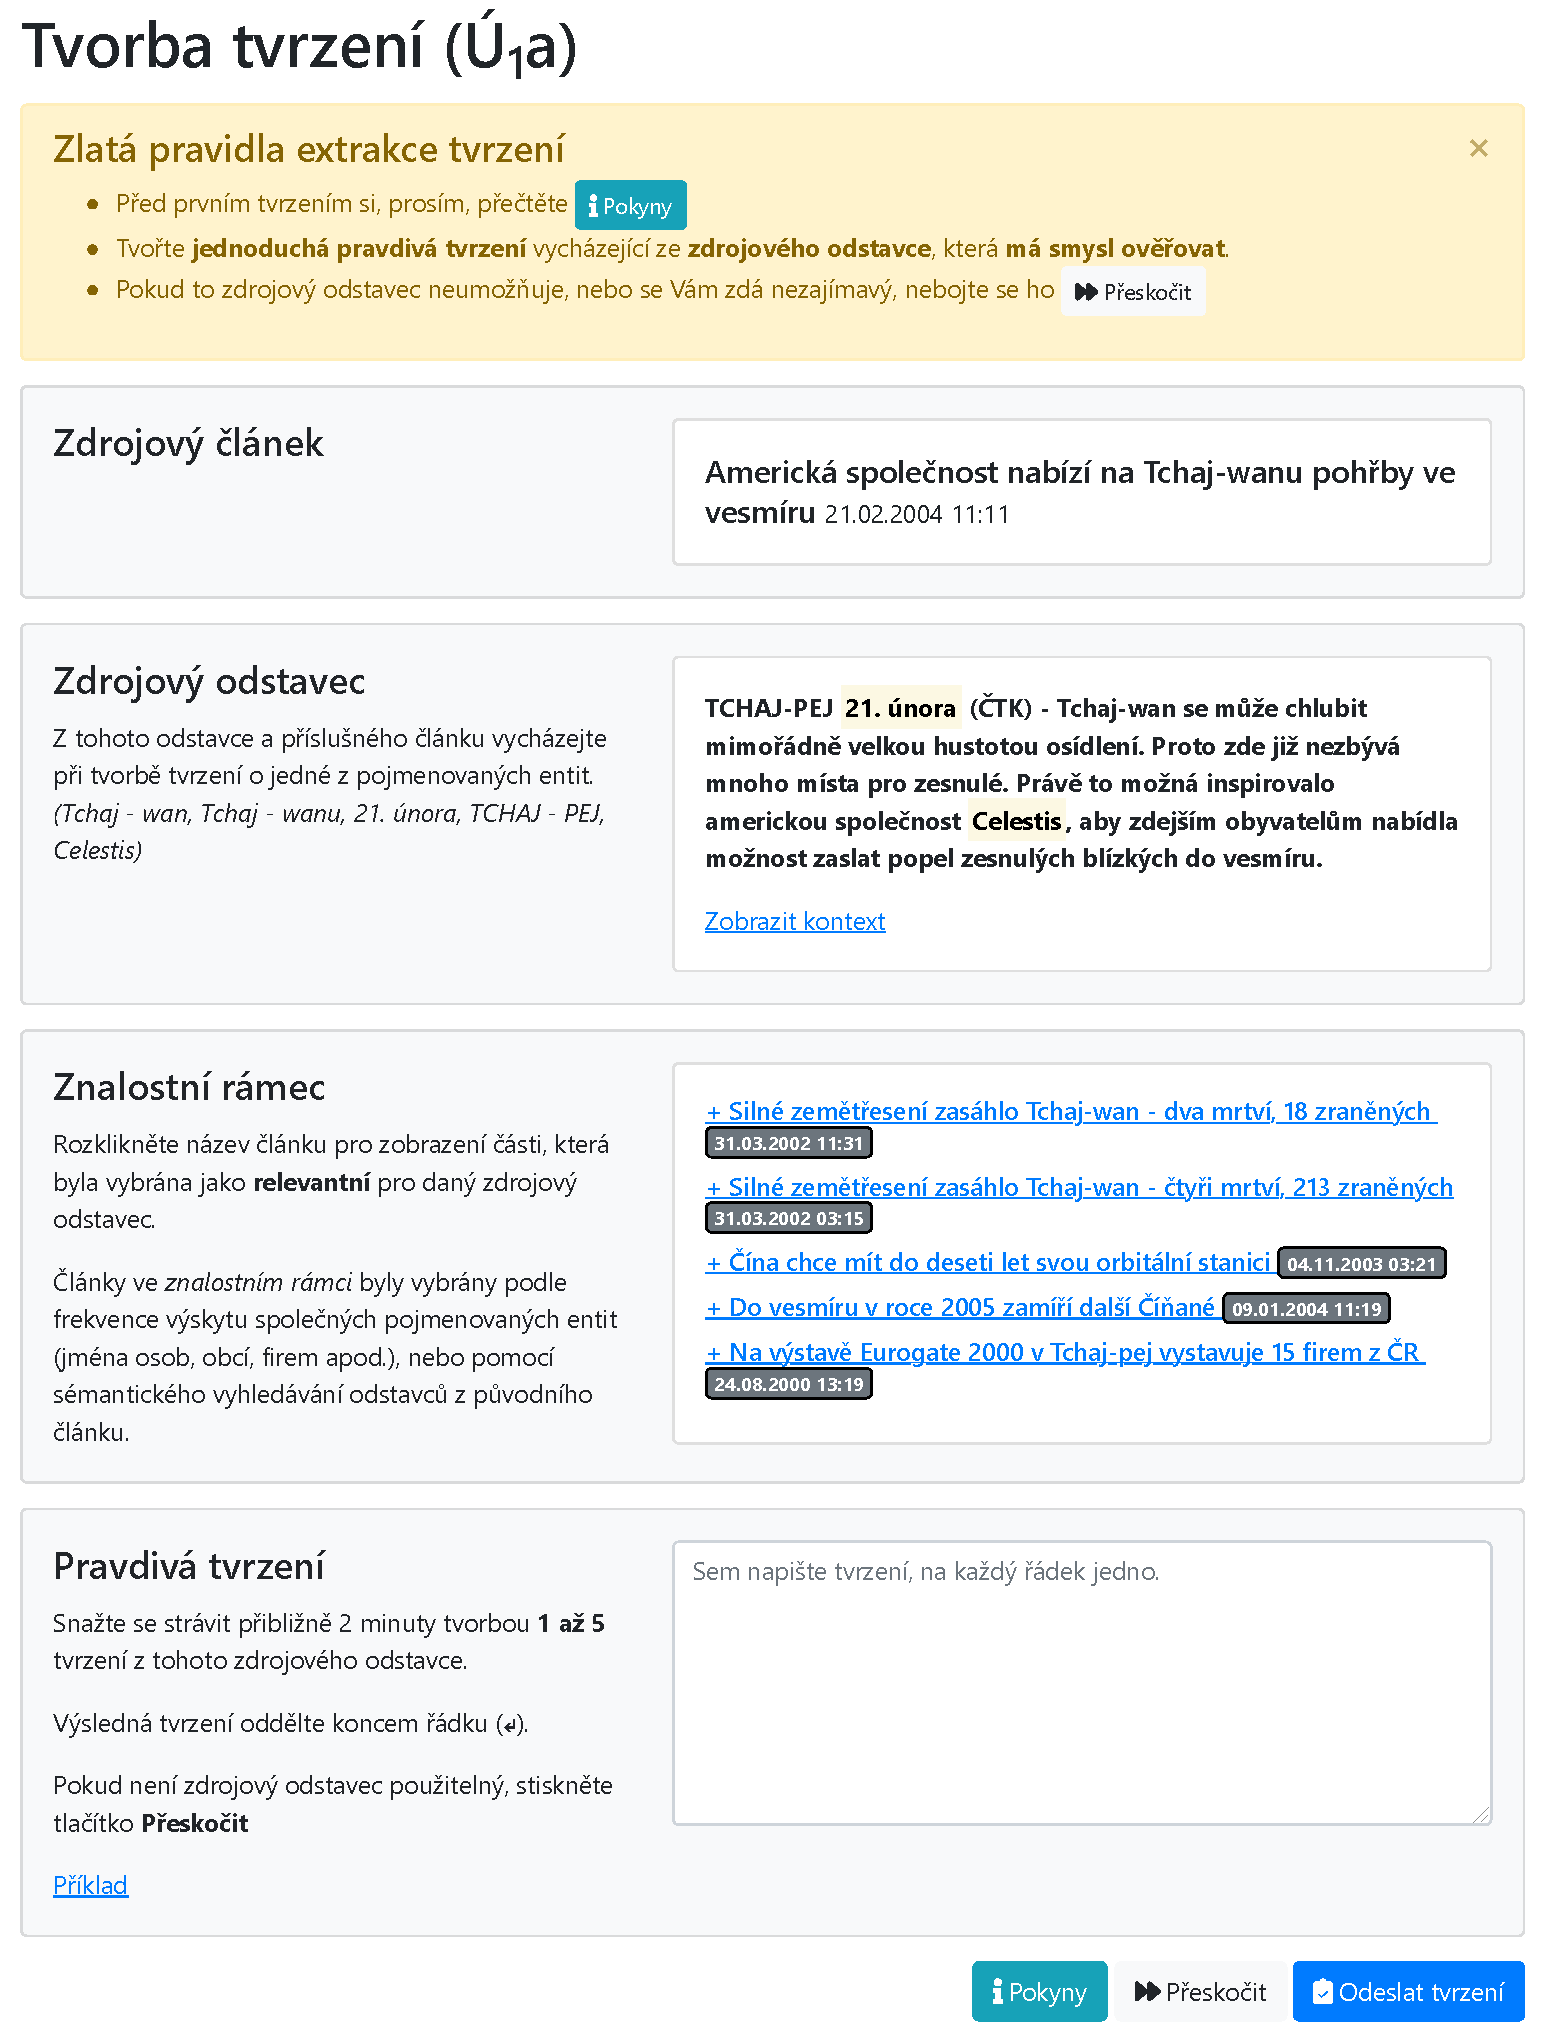
\includegraphics[width=19cm]{fig/claim_extraction.pdf}}}
\label{fig:extraction}
\caption[Claim extraction interface of \textsf{FCheck} platform]{Claim extraction interface of the \textsf{FCheck} platform}%Full English translation attached as Figure~\ref{trans:extraction} TODO: Friday
\end{figure} % Extraction
\pagebreak
\begin{figure}[H]
\thispagestyle{empty}
\vspace{-2cm}
 \makebox[\textwidth][c]{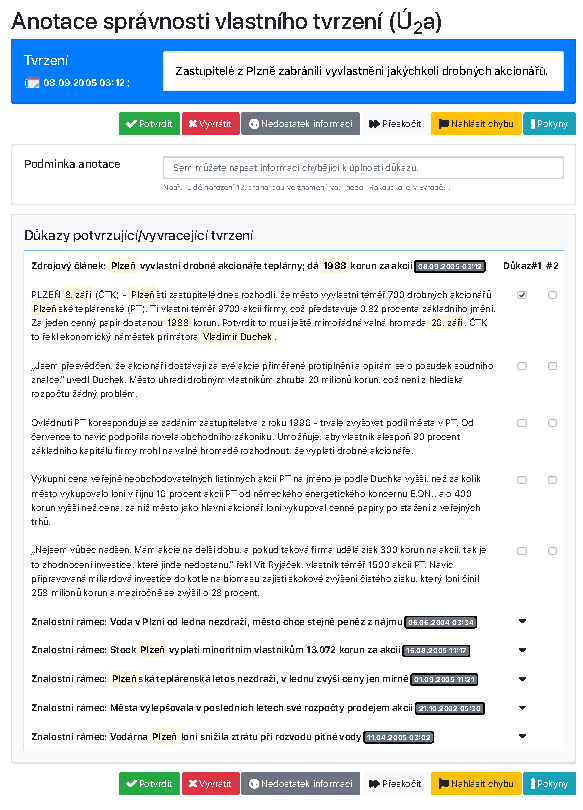
\includegraphics[width=18cm]{fig/annotation.pdf}}

\caption[Claim labelling interface of \textsf{FCheck} platform]{Claim labelling interface of \textsf{FCheck} platform. Full English translation attached as Figure~\ref{trans:annotation}}

\label{fig:annotation}
\end{figure} % Mutation
\pagebreak


\subsection{Claim Veracity Labeling}
\label{sec:ui-labeling}
In Figure~\ref{fig:annotation} we show the most complex interface of our platform -- the \tdva{}: \textbf{Claim Annotation} form. 

Full instructions take about 5 minutes to read and understand, and are hid away in the \btn{Instructions} modal window, that is to be opened during the first annotation, and the on demand. All actions are spread out on the top bar and \textit{label condition} is collected through a text field above the evidence input. This was decided after a negative experience with using a modal \btn{Actions} to hide away less frequent actions, originally inspired by other annotation platforms (see~\ref{sec:flat}).

The input of multiple evidence sets works as follows: each column of checkboxes in~\ref{fig:annotation} stands for a single evidence set, every paragraph from the union of knowledge belongs to this set iff its checkbox in the corresponding column is checked. Offered articles \& paragraphs are collapsible (without loss of checkbox state), empty evidence set is omitted. Through \textsf{JavaScript}, interface always displays all the non-empty sets defined so far, plus one empty column of checkboxes that can be used to initialize a new one.

On average, the labelling task took \textbf{65 seconds}, with a median of \textbf{40s}. An average \texttt{SUPPORTS}/\texttt{REFUTES} annotation was submitted along with \textbf{1.29} different evidence sets, 95\% of which were composed of a single paragraph -- full histograms will be introduced in Chapter~\ref{chap:dataset}.


\section{Between-Wave Platform Adjustments}
 \textit{\textit{Annotation wave} is our term for a group of \textsf{FSS} students annotating towards a common deadline, for a fixed period of 10--14 days.}
 
 \textit{To date, have supervised a total of a 4 annotation waves, however, as the wave 3 and 4 were largely simultaneous and their deadlines only differed in two days, we group them together as the \textit{$3^{rd}$ wave (Figure~\ref{fig:performance})}.}
 
  \begin{figure}[H]
\makebox[\textwidth][c]{{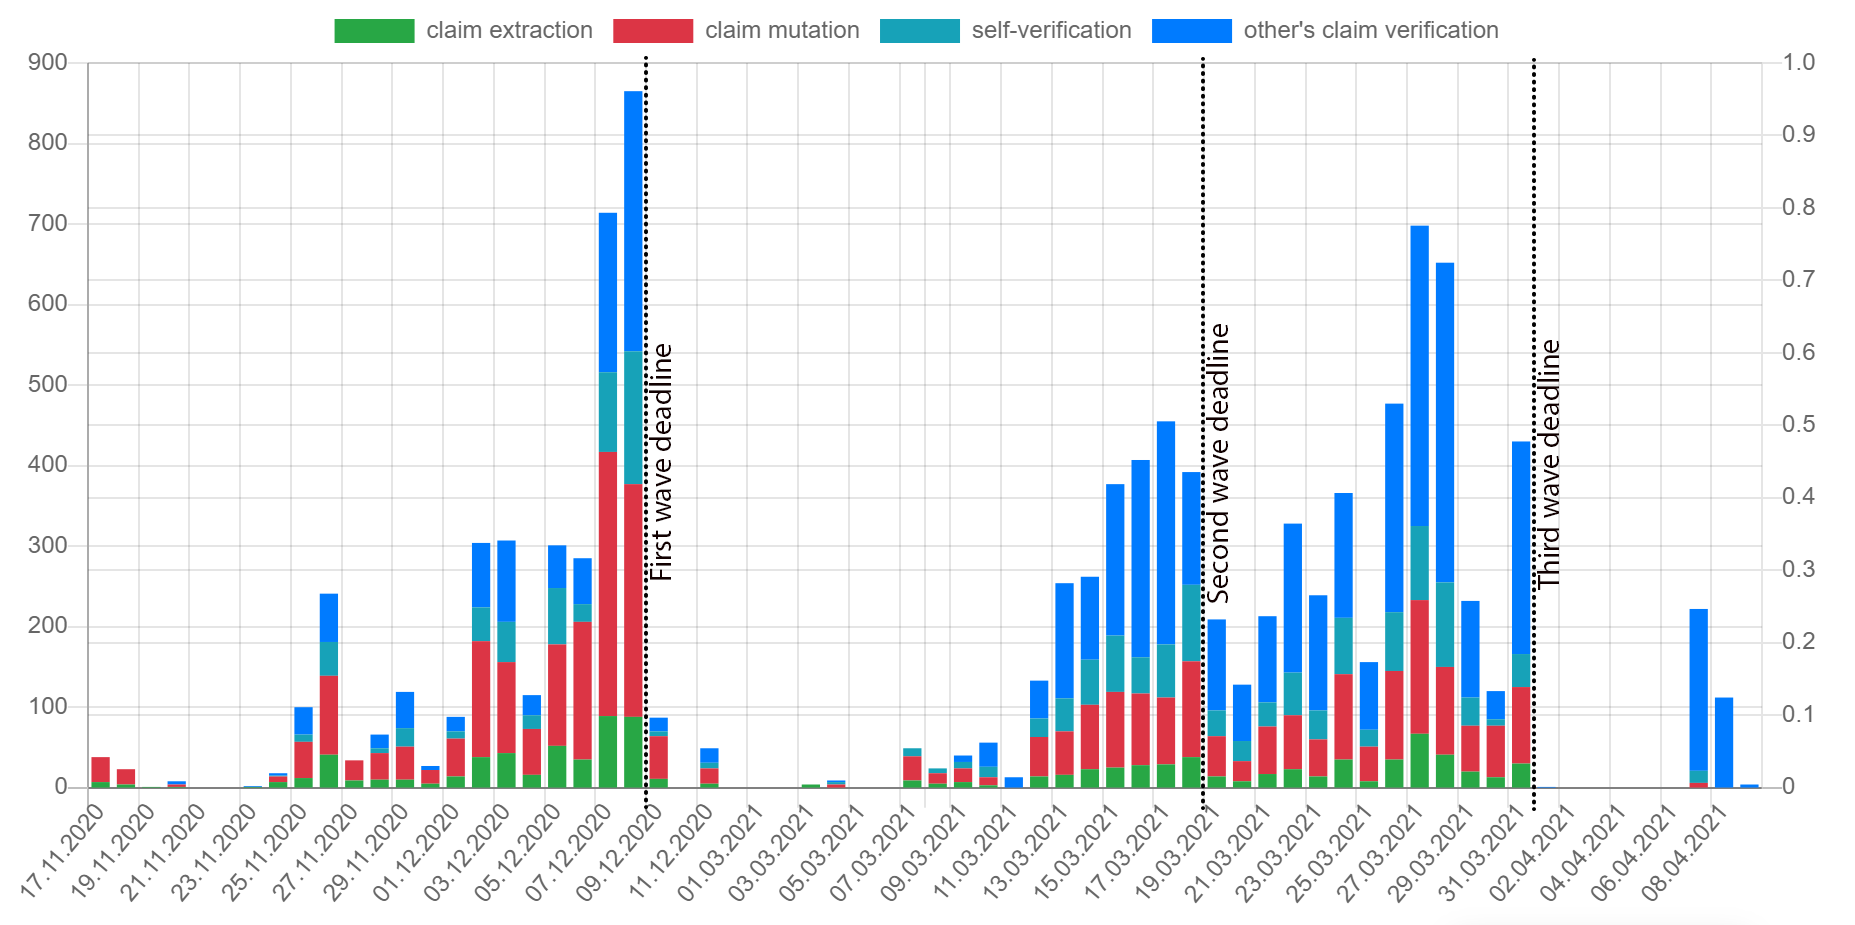
\includegraphics[width=18cm]{fig/performance.png}}}
\caption{Number of data points generated per day, colored by task}
\label{fig:performance}
\end{figure} % pestrobarevny graf
 
 Thanks to the multi-wave system of annotation, we were able to utilize our findings from the live data directly to patch the deployed version of the \textsf{FCheck} platform. This was particularly useful between the $1^{st}$ and the $2^{nd}$ wave. Here are the adjustments we presented, based on the learnings from the data exploration:


\subsection{The Golden Rules of Each Task}
\label{sec:golden-rules}
To address the most frequently reoccurring annotation errors, which will be examined in depth in Chapter~\ref{chap:dataset}, we have came up with a set of guidelines for each task. However, we found that the annotators tend to never re-read the full \btn{Instructions}, and to forget some of the important guidelines over time. Therefore, we have limited ourselves to 3 \textit{golden rules} per task, that will be present all the time, directly in the annotation task screen.


\begin{enumerate}
        \item[\itembox{\tjednaa{}}] \textbf{Golden Rules of the Claim Extraction:} 
        \begin{enumerate}
            \item[\itembox{1.}] Please read the \btn{Instructions} before making your first claim.
            \item[\itembox{2.}] Make \textbf{simple true claims} based on the source paragraph that\textbf{ make sense to be verified}.
            \item[\itembox{3.}] If the source paragraph doesn't allow that or seems uninteresting, feel free to \btn{Skip} it.
        \end{enumerate}
        \item[\itembox{\tjednab{}}] \textbf{Golden Rules of the  Claim Mutation:}
        \begin{enumerate}
            \item[\itembox{1.}] Please read the \btn{Instructions} before making your first mutation.
            \item[\itembox{2.}] {\techbf !} \textbf{Only make mutated claims that make sense to be verified.}
            \item[\itembox{3.}] Therefore, there is no need to use all 6 mutation types, 3 would suffice, even 1.
        \end{enumerate}
        \item[\itembox{\tdva{}}] \textbf{Golden rules of the Claim Annotation}: 
        \begin{enumerate}
            \item[\itembox{1.}]Before the first annotation, please, read the  \btn{Instructions}.
            \item[\itembox{2.}]Pay attention to \textbf{the non-exclusivity of phenomena}, especially for the \btn{Refute} annotations. \textit{E.g. \"{a cinema is being built in Písek} does not refute \"{a gallery is being built in Písek}}.
            \item[\itembox{3.}] If the evidence alone is not sufficient, please provide the missing information as a \textit{condition} of the annotation.
        \end{enumerate}
    \end{enumerate}
    
\subsection{T2: The Action Flattening}
\label{sec:flat}
After the first wave of annotation, that showed  a significantly underwhelming usage of \tdva{} actions grouped in an \btn{Actions} modal pop-up -- especially the usage of the \texttt{NOT ENOUGH INFO} label, \btn{Flag}s and \textit{conditions} -- we have re-thought the action toolbar and spread all the actions available onto a horizontal bar, each as a single button. If the action requires additional data, s. a. the \btn{Flag} reason, it only asks for it in a \"{next step} modal window.

\subsection{T2: User-Initiated Soft-Deletion}
\label{sec:soft-deletes}
In addition to this, we have added the feature of \textit{soft-deletes}. Thanks to the convenience of working with the \textsf{Yii2 PHP} Framework, we could simply constrain the system to only work with entity objects without the soft-deletion bit set to \texttt{1}, effectively augmenting each query above such an entity with \"{(\dots) \texttt{WHERE} (\dots) \texttt{AND deleted!=1}}.

Since the Wave 2, each \btn{Flag} was programmed to cause a temporary soft-delete of the flagged claim, to be re-considered by an administrator. This has shown to be a great synergy of the human-power of the annotators and admin's unconstrained system access. Admin got notified every time there was a claim containing a typo, a contradiction, or claim unrelated to the source paragraph, and did his best to fix the claim using his direct \textsf{db} access. In the meantime, the claim was inaccessible to the web user interface, and no annotation was wasted on invalid data. 

Over the waves 2 and 3, we have received a total of \textbf{112} flags, effectively saving almost \textbf{4 hours} of compromised annotation, estimated using the average \tdva{} load (\ref{sec:ui-labeling})  and 2 cross-annotations per claim. We have managed to recover \textbf{65} of the flagged claims to a state valid for the annotation task.

\subsection{Spreading out the annotations}

During the first wave, we have experienced a severe peak in annotators performance during the deadline (Figure~\ref{fig:performance}). As relatable as that sounds, it did have a bad impact on the dataset quality.

\begin{figure}[H]
\makebox[\textwidth][c]{{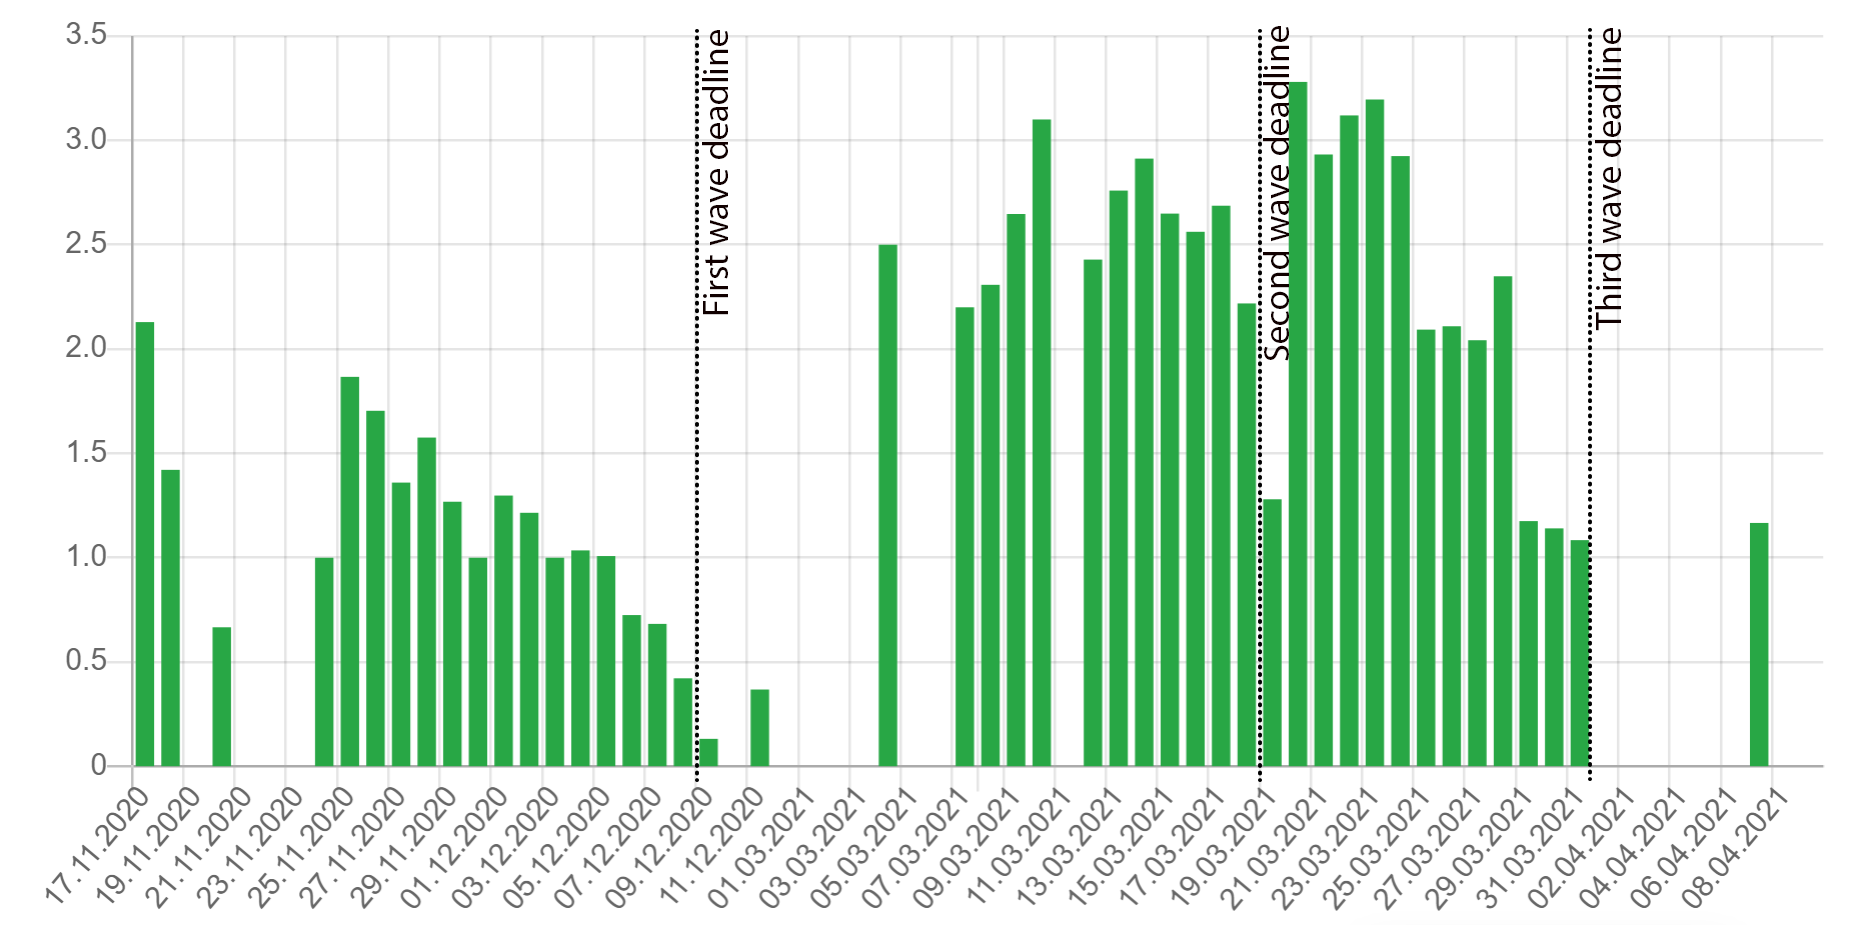
\includegraphics[width=18cm]{fig/number-of-crossannotations.png}}}
\caption[Average number of cross-annotations per claim by day]{Average number of cross-annotations per claim by day. Only counting annotations within the current wave (+2 days tolerance -- not showing the post-wave adjustments).}
\label{fig:crossannotations}
\end{figure} % zeleny graf

Due to the unbiased claim sampling in \tdvab{}, the late claims were extremely punished, as they were absent for most of its instances. The Figure~\ref{fig:crossannotations} shows this phenomenon -- on December $8^{th}$ the average number of annotations per claim descended below 0.5, which is very unfortunate, as the Figure~\ref{fig:performance} shows this day to be the second most productive in the claim mutation.

Therefore, we have biased the \tdva{} claim sampling in the following ways:
\begin{enumerate}
    \item $m^c$ is assigned a random priority from $(0,1)$
    \item If $m^c$ comes from the current wave of annotation, priority is incrementated by 1 
    \item If $m^c$ has less then 1 non-oracle annotation\footnote{Originally, we have tried to aim for 2 non-oracle annotations per claim, however, this was too punishing for the unannotated claims left from previous waves, as each new claim would be favoured for as long as it does not collect 2 annotations}, priority increments by 1
    \item Finally, $m^c$ with the highest priority is sent on output.
\end{enumerate}

Fast implementation of this sampling using the \textsf{SQL} \textit{subqueries} can be found in the attached  \texttt{LabelController.php}.

In addition to this, we have \textbf{adjusted the required number of data-points per task}.
From 5 \tjednaa{} claims, 15 \tjednab{} mutations, 5 \tdvaa{} oracle annotations and 15 \tdvab{} non-oracle annotations, we have switched to\textbf{ 3, 7, 7} and \textbf{35}, respectively (Figure~\ref{sec:workflow}), based on our stopwatch-per-task measurements and the findings from Figure~\ref{fig:crossannotations}, in which the $1^{st}$ \textit{Wave} partition shows the need for an increase in cross-annotations.

Lastly, we have dedicated the time to hand-annotate\textbf{ \char`~300 residual claims} after the last wave. These adjustments led to a significant improvement over the random baseline -- for instance, after the first wave deadline, around 40\% of all claims ended up with 0 annotations. By the time of the publication of this thesis, the amount of the 0-annotated claims decreased to only 9\%, still counting the original $1^{st}$ wave set, subject to its post-annotations.


\section{System Performance Remarks}
We have been surprised by the robustness and traffic resistance of the resulting scheme. Dataset does not contain traces of blackouts or \texttt{HTTP} communication interrupts between \textsf{Flask} and \textsf{Apache}. We also consider the traffic load carried by our system during the wave deadlines (Fig~\ref{fig:performance}) remarkable, given the size of the \textsf{ČTK Archive} and the complexity of the~\ref{sec:knowledge-scopes} algorithm. We attribute this to the full \textsf{AJAX}-initiated asynchronization of the costly operations and to the support we recieved from the \textsf{Faculty of Electrical Engineering}, namely Petr Benda, who provided us with a server with \textsf{Intel Xeon E3 CPU} and 132 GB of memory that runs both \textsf{Flask} and \textsf{Apache} apps to this date\footnote{As of May 20$^{th}$}.

\section{Annotation wrap-up}
We have successfully conducted three experiments on human annotation for the \textit{fact-checking using \textsf{ČTK Archive}} task, using a novel annotation platform of our own design, which is \textit{live} on \url{https://fcheck.fel.cvut.cz}, or can be installed from its source\footnote{\url{https://gitlab.fel.cvut.cz/factchecking/fcheck-anotations-platform}} that is to be published under a license to be specified in \texttt{LICENSE.md}.

We thank to all \textsf{FSS} students who participated in our experiments for donating their time to support our endeavours with a total of \textbf{4,325} valid \db{Claim}, and \textbf{5,759} \db{Label} datapoints.
According to their verbal feedback after the supplementary lectures, many of them enjoyed our cooperation\footnote{Even if, based on the textual inputs found in our database, at least one did not}, and the research partnership started with our project shall continue with other exciting future collaborations. 

%%!TEX ROOT=../ctutest.tex

\chapter{ČTK Dataset Analysis and Postprocessing}
\label{chap:dataset}

Through the methodology described in chapter~\ref{chap:ctk}, we have collected a set of raw claims and samples of their veracity labelling.

This chapter performs the exploratory analysis of the collected dataset, structured as described with Figure~\ref{fig:er}, and describes our methods of \"{flattening} it into a single text file that is easy to parse. Consecutively, we analyse the resulting dataset using several standard metrics and propose tools for its iterative refinement, ultimately leading to the current version of \textsf{ČTK} dataset, described and linked in~\ref{sec:dataset-latest}.

\begin{figure}[H]
\makebox[\textwidth][c]{{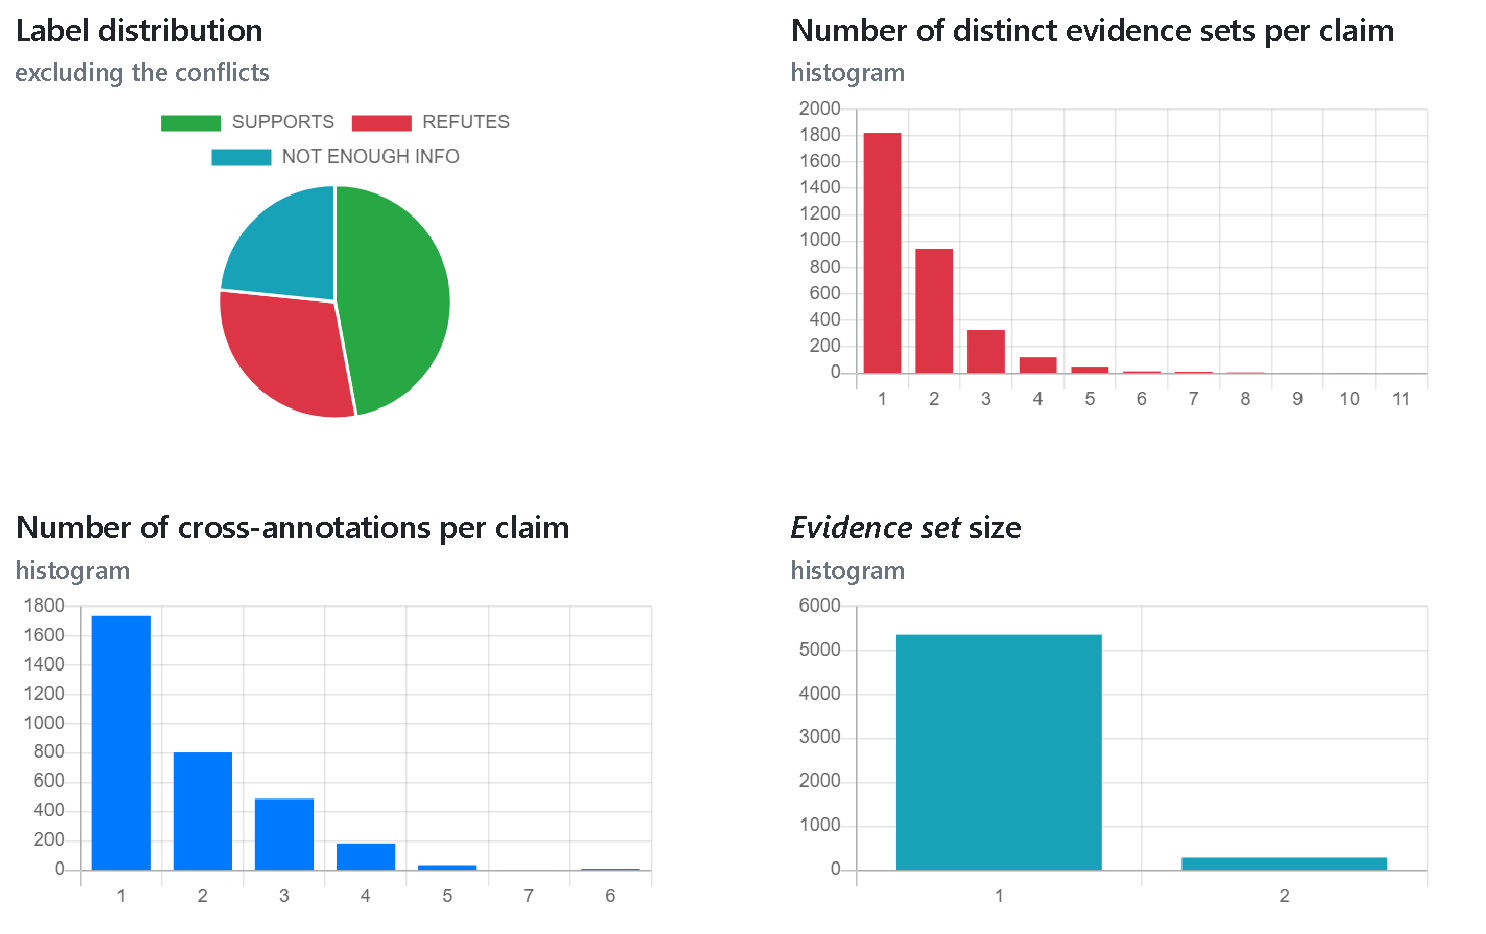
\includegraphics[width=16cm]{fig/dashboard.pdf}}}
\caption[Visualizations of properties of the collected dataset]{Visualizations of properties of the collected dataset, extracted from our interactive dashboard (Section \ref{sec:dashboard}) attached to this thesis.}
\label{fig:dashboard}
\end{figure} % zeleny graf

\section{Live Dashboards}
\label{sec:dashboard}
In order to provide our users with a comprehensible view into the resulting dataset and its properties, including the leaderboard of the most active annotators, we have implemented a dashboard of \textit{live} data visualizations. For the live data aggregations, we have mostly used raw \textsf{PHP} and \textsf{SQL}, for interactive and \ae{}sthetically pleasing plots, we have used the \textsf{Chart.js} library.

We have decided to disclose the dashboard (with supplementary labels in Czech) to our reader, so as to accompany the texts to follow, and to provide a legible statistical insight into the data collected by the methods listed in Chapter~\ref{chap:ctk}.

It can be found at \url{https://fcheck.fel.cvut.cz/site/statistics} and logged into using the \"{\texttt{testuser}} \textsf{SIDOS ID}.

\section{JSON Lines FCheck Export}
\label{sec:export}
For the purpose of \textit{flattening} the \textsf{FCheck} database with all of its relations and metadata to a single concise text file used on an input for our end applications, we have constructed a \textsf{JSONL API} at \texttt{https://fcheck.fel.cvut.cz/label/export}.

It takes the following arguments through its \textsf{HTTP GET} parameters:
\begin{enumerate}
    \item \texttt{shuffle} $\in\{\texttt{0},\texttt{1}\}$, defaults to \texttt{0}\\ decides, whether the dataset should be shuffled using the \textsf{MySQL}'s \dots\texttt{ORDER BY rand()}
    \item \texttt{evidenceFormat} $\in\{\texttt{text},\texttt{ctkId}\}$, defaults to \texttt{ctkId}\\
    if set to \texttt{text}, the full detokenized text of used \textsf{ČTK} paragraphs will be exported for evidence (preferred for NLI), otherwise, only the underscore-separated article and paragraph id will be given, s.a. \texttt{T201810060771501\_2} (preferred for DR)
    \item \texttt{summer} $\in\{\texttt{0},\texttt{1}\}$, defaults to \texttt{0}\\ decides, whether the first wave of annotations  should be excluded from the export, by default it is sorted by the source paragraph
    \item \texttt{fever} $\in\{\texttt{0},\texttt{1}\}$, defaults to \texttt{0}\\ switches to the \textsf{FEVER}-like output format (\ref{list:fever}), to ease the usage of \textsf{FCheck} data for experiments implemented to run with \textsf{FEVER CS} -- setting to \texttt{1} disables the other options for legacy reasons
\end{enumerate}

\subsection{ČTK dataset formats}
While much like~\cite{fever} we use the \textsf{JSONL} file type, which we deem appropriate for the fact verification datasets, we propose an alternate format for flattening the data points than that from Figure~\ref{list:fever}. In our case, we argue to suppress all the auxiliary information except the \db{Claim} \texttt{id} to refer back to the \ref{fig:er} representation of data, following the KISS\footnote{\"{Keep It Simple, Stupid!}} and YAGNI\footnote{\"{You Ain't Gonna Need It.}}~\cite{jeffries2001extreme} design principles.

While this interpretation of the \textit{labeled-claim} datapoints is our current default, we also enable switching back to the \textsf{FEVER} format illustrated in~\ref{list:fever}, using the \texttt{fever} flag for backwards compatibility. This is particularly useful for reusing the model training procedures written for \textsf{FEVER CS}. 

We demonstrate the two types of \db{Evidence} representation in Figures~\ref{list:fcheck-ctkid} and~\ref{list:fcheck-text} -- \texttt{text}  is meant for the training and validation of the NLI models (Chapter~\ref{chap:nli}), whereas \texttt{ctkId} suits the Retrieval tasks. For the completeness, the \texttt{ctkId} consists of the \textsf{ČTK Archive} identifier and the paragraph 1-based index in the archived article, separated by underscore. Index 0 is reserved for the article headline as it may also be used for both tasks.

\begin{figure}[H]
\begin{lstlisting}[language=json]
{
  "id": 2500,
  "label": "SUPPORTS",
  "claim": "S Dejvickým divadlem spolupracoval Petr Zelenka.",
  "evidence": [
    ["T201111230392601_9"],
    ["T200708140695001_2"]
  ]
}
\end{lstlisting}
    \caption[Example of \textsf{ČTK} datapoint, \texttt{ctkId} evidence format]{Example \textsf{ČTK} \texttt{SUPPORTS} annotation with two possible evidence sets, each composed of one \textsf{ČTK} paragraph, using the \texttt{ctkId} evidence format.}
    \label{list:fcheck-ctkid}
\end{figure}
\begin{figure}[H]
\begin{lstlisting}[language=json,escapeinside={(*}{*)}]
{
  "id": 2500,
  "label": "SUPPORTS",
  "claim": "S Dejvickým divadlem spolupracoval Petr Zelenka.",
  "evidence": [
    ["Petr Zelenka vystudoval scenáristiku a dramaturgii na FAMU (*(\dots)*) V roce 2001 napsal pro Dejvické divadlo (*Příběhy*) (*obyčejného*) šílenství, za které získal Cenu Alfréda Radoka (*(\dots)*)"],
    ["(*(\dots)*) kterou Zelenka (*později*) (*režíroval*) i jako stejnojmenný film. V roce 2005 uvedl na dejvické (*scéně*) svou (*další*) hru Teremin. V (*současné*) (*době*) (*natáčí*) Zelenka osobitou verzi inscenace Dejvického divadla Karamazovi."]
  ]
}
\end{lstlisting}

    \caption[Example of \textsf{ČTK} datapoint, \texttt{text} evidence format]{The same example as~\ref{list:fcheck-ctkid} using the \texttt{text} evidence format, paragraphs were truncated using \texttt{(\dots)}}
    \label{list:fcheck-text}
\end{figure}
\begin{figure}[H]
\begin{lstlisting}[language=json,escapeinside={(*}{*)}]
{
  "label": "SUPPORTS",
  "claim": "S Dejvickým divadlem spolupracoval Petr Zelenka.",
  "context": [
    "(*(\dots)*) Petr Zelenka (*(\dots)*) napsal pro Dejvické divadlo (*(\dots)*)"
  ]
}
\end{lstlisting}

\begin{lstlisting}[language=json,escapeinside={(*}{*)}]
{
  "label": "SUPPORTS",
  "claim": "S Dejvickým divadlem spolupracoval Petr Zelenka.",
  "context": [
    "(*(\dots)*) kterou Zelenka (*(\dots)*) 2005 uvedl na dejvické (*scéně*) (*(\dots)*) "
  ]
}
\end{lstlisting}

    \caption[Example of \textsf{ČTK} datapoint, \texttt{nli} evidence format]{The same example as~\ref{list:fcheck-text} using the \texttt{nli} evidence format, paragraphs were truncated using \texttt{(\dots)}. Note that in this format we have 2 datapoints - one for each evidence set.}
    \label{list:fcheck-nli}
\end{figure}

Additionally, we introduce the \textsf{ČTK} \texttt{nli} format that is appropriate for training and testing the Natural Language Inference models in the Figure~\ref{list:fcheck-nli}, note that this format produces a different number of datapoints, one for every evidence set, listed as \texttt{context}.



\section{Cross-annotations}
\label{sec:cross-annotations}
In \textsf{FEVER} annotation labeling task \textsf{WF2}~\cite{fever}, the annotators were advised to spend not more than 2-3 minutes to find as many of the evidence sets as possible in the given dictionary (and even using a direct \textsf{Wiki} access), so that the dataset can later be considered \textit{exhaustive}, i.e., to boost its \textit{evidence recall}, which was later computed to be \textbf{72.36\%}.

With our \textsf{ČTK Archive} corpus, this is unrealistic, as it commonly contains an inconceivable number of copies for a single ground truth\footnote{Think, the proposition \"{Miloš Zeman is the Czech president}, which can be found in every \"{(\dots), said the Czech president Miloš Zeman.}}. So is the number of paragraphs in the \textit{mutated claim}'s knowledge scope, typically close to (see \tjednab{} and \ref{sec:knowledge-scopes} for reference) $\text{max}_{m^c}|knowledge(m^c)\cup knowledge(p) \cup\{p\}|=17$. Therefore, we proposed a different scheme: we advised every annotator to spend 2-3 minutes finding a \textit{reasonable} number of distinct evidence-sets, w.r.t. the time needed for a good reading comprehension. Furthermore, we randomly shuffled the set of all \textit{knowledge scope} documents using \textsf{PHP}'s \texttt{shuffle}\footnote{Which internally uses the Mersenne Twister pseudorandom number generator, for the completeness} before the start of every \tdva{} annotation.

As the annotators typically skim through the knowledge headlines in a top-first order, this made it difficult for two annotators to arrive to the same set of evidence-sets. To exploit that, we collected multiple \textit{cross-annotations} for each claim -- their distribution is best visualized with the histograms in Figure~\ref{fig:dashboard}. Finally, as a subroutine of our export tool~\ref{sec:export}, we merge the evidence of all the cross-annotations for a given claim together, to achieve the highest possible \textit{recall}.


\section{Inter-Annotator Agreement}
A desirable byproduct of the cross-annotation-driven approach above are the large resulting groups of $k$-way \textit{labeled} claims. I.e., the claims that were assigned exactly $k$ independent labels from $\{\texttt{SUPPORTS},\texttt{REFUTES},\texttt{NEI}\}$ by different annotators.

To measure the agreement using the most straightforward implementations of the measures enumerated in Table~\ref{tab:agreement-metrics}, we first conclude two \textit{pairwise} agreement experiments, first using the average 0/1-agreement measure (listed as the \%-aggreement), then the Cohen's~$\kappa$~\cite{cohen}, which is the standard for bipartite agreement. By \textit{pairwise experiment}, we mean an exp't concluded using the enumeration of all the pairs of labels of every $(\geq 2)$-way labeled claim on its input.

Secondly, we examine each $k$-way annotated partition of claims using the Fleiss' $\kappa$ measure introduced in~\cite{fleiss}, which is the standard for the $k$-way inter-annotator aggreement. We list its results on the most significant $(>2)$-way-annotated partitions of our dataset, along with the share of the partition in the whole dataset, denoted as the \textit{Claim-Coverage}.

\begin{center}
\begin{table}[H]
\begin{ctucolortab}
\begin{tabular}{ l | c | l | c }
Metric & Value & Agreement\tablefootnote{The verbal interpretation is provided for reader's convenience and follows the interpretation tables of~\cite{legend} which are mainly orientational and by no means universally accepted.} & Claim-Coverage\tablefootnote{The percentage of labeled claims eligible for this experiment out of the entire set.}  \\
\hline
{ Pairwise percent agreement} &\textbf{74\% }& ~ & 55.9\% \\
{ Pairwise Cohen's $\kappa$} &\textbf{0.58} & \textit{moderate}& 55.9\% \\
{ 3-way Fleiss' $\kappa$} & \textbf{0.57}  & \textit{moderate}& 19.3\%\\
{ 4-way Fleiss' $\kappa$} & \textbf{0.63} & \textit{substantial} & 7.5\%\\
{ 4-way Krippendorff's $\alpha$} & \textbf{0.63} & \textit{substantial} & 7.5\%\\
{ 5-way Fleiss' $\kappa$} & \textbf{0.61} & \textit{substantial} & 1.7\%\\
\end{tabular}
\end{ctucolortab}
\caption{Inter-annotation agreement metrics of the \textsf{ČTK v2.1} dataset, excluding the \textit{conditional annotations}}
\label{tab:agreement-metrics}
\end{table}
\vspace{-2.5em}
\end{center} 

\textit{Experimentally, we have also calculated the Krippendorff's $\alpha$ from~\cite{krippendorff2013content}, which yielded the same results as the Fleiss' $\kappa$ up to 2 decimal spots. Krippendorff's $\alpha$ should be appropriate for the agreement experiments with missing data, measuring the within- and between-unit error. We encourage a further experimentation using Krippendorff's $\alpha$ and the entire \textsf{ČTK} dataset augmented by the annotator identifiers in the future.}

~

The measurements can be replicated using the attached \texttt{agreement.py} \textsf{Python} module and the cross annotation May'21 snapshot in \texttt{cross\_annotations.csv}. We consider the results promising with respect to the complexity of the \tdva{} task and the \textsf{ČTK} corpus. To put in context, \cite{fever} achieved a 5-way Fleiss' kappa of \textbf{0.68} using a simpler \textsf{ENWiki} dataset, dictionary structure and longer total time per annotator, affecting the \textit{learning curve}. \cite{danish} demonstrated the importance of this factor by achieving \textbf{0.75} $\kappa$-score through only using two expert-level annotators -- themselves. We conclude that the dataset is usable for the fact-verification task, which we will demonstrate on its NLI subroutine (Chapter~\ref{chap:nli}).


\subsection{Annotation Cleaning}
\label{sec:cleaning}
We have dedicated a significant amount of time to manually traverse \textit{every} disagreeing pair of annotations, to see if one or both of them violate the annotation guidelines. The idea was that this should be a common case for the conflicting annotations, as the \textsf{ČTK News Archive} corpus does not commonly contain a conflicting pair of paragraphs except for the case of \textit{temporal reasoning} shown in Chapter~\ref{chap:ctk}. In the same chapter, we have resolved this case using the \textit{claim timestamps}, that always favour the latest knowledge published up to the given date.

Indeed, after separating out the incorrectly formed annotations using our \textit{soft-deletion} mechanisms introduced in the section \ref{sec:soft-deletes}, we have been able to resolve every conflict, ultimately achieving a \textit{full agreement} between the annotations. However, the metrics listed in Table~\ref{tab:agreement-metrics} do \textit{not} exclude the soft-deleted labels, so as to provide a better insight into the reliability of the data \textit{without} the conflict.

%\section{Precision/recall Against Oracle Annotations}
\section{Common annotation problems}
\label{sec:annot_problems}
After removing hundreds of ineligible annotations in~\ref{sec:cleaning}, we would like to mention several archetypes of their underlying problems. Their avoidance should be put into cosideration when designing similar annotation experiments in the future.
\begin{enumerate}
    \item {\techbf{Exclusion misassumption}} -- by far the most prevalent type of misclassification: the annotator uses a ground truth independent of the claim as a \texttt{REFUTES} evidence. E.g., \textit{\"{Postoloprty opened a new cinema} \texttt{REFUTES} \"{Postoloprty opened a new museum}}.
    
    While on the first sight, this might seem like a sound disproof, there is no textual entailment between the claims nor their negations. We attribute this error to confusing the \tdva{} with a \textit{reading-comprehension}\footnote{\textit{\"{Does the article tell us that Postoloprty opened a museum? Highlight the relevant information.}}} task common for the field of humanities.
    
    We have reduced the frequency of this misclassification by introducing a \textit{golden rule} (Section~\ref{sec:golden-rules}) for it, keeping it on annotator's mind at all times
    \item {\techbf{Mutation vagueness}} -- \db{Claim} fault. Mutation generalizes out an integral part of the original claim, typically the named entities. E.g., $m^c=\text{\"{The convoy is 200 metres long}}$ 
    \item {\techbf{Temporal reasoning}} -- an inherent problem of the journalistic datasets -- an annotater submits a dated evidence paragraph that contradicts the latest news w.r.t. $timestamp(m^c)$
    \item {\techbf{NEI "shyness"}} -- \"{Pandas are endangered.} was used once for \texttt{SUPPORTING} and once for \texttt{REFUTING} the claim \"{Koalas are endangered.}, zero times as \texttt{NEI}.  This, among other examples, shows that our annotators often preferred the \textit{definite} labels, even where \texttt{NEI} is appropriate, which might justify its underrepresentation shown in Figure~\ref{fig:dashboard}.
    
    We tried to address this introducing the \textit{conditional} annotations (Section~\ref{sub:conditional}).
\end{enumerate}

 For the completness, we attach the raw file \texttt{archetypy.docx}\footnote{\url{http://bertik.net/archetypy.docx}} in Czech, naming multiple examples from \textsf{ČTK v1} dataset for each of the archetypes above.

\section{Legacy version notes on the ČTK dataset}
As there were several different export snapshots of our data used for the experiments in Chapter~\ref{chap:nli} and the work of~\cite{rypar}, we include version notes for the major dataset versions to refer back to:

\begin{itemize}
    \item {\techbf ČTK dataset v1} -- December 2020
    
    Legacy dataset published in the \textsf{FEVER} format (\ref{list:fever}), featured the first wave of \textbf{\char`\~950} annotations, highly experimental, significantly helped to reveal the data faults described in the Section~\ref{sec:annot_problems}.
    
    \item {\techbf{ČTK dataset v2}} -- April 2020
    
    Cleaned (\ref{sec:cleaning}). Contains the first snapshot of data from all three waves, ignoring \textit{conditional annotations} and conflicts. Follows the label distribution from Figure~\ref{fig:dashboard} using a \textit{stratified} \textsf{train-dev-test} split generated through two iterations of \textsf{scikit-learn}'s \texttt{train\_test\_split}, each with a fixed \textit{random seed} and a test size of 0.2
    
    \item {\techbf ČTK dataset v2csv}
    \label{item:ctk-csv}
    
    Generated in parallel as a part of Jan Drchal's research from the May snapshot of \textsf{FCheck db}. It attempts to minimize the \textit{document leakage}~\ref{sec:leakage} by sorting the claims by their source paragraph before the \textsf{train-dev-test} split. Ignores the evidence grouping (\ref{fig:er}), however, yields encouraging results for NLI.
    
    \item {\techbf ČTK dataset v*nli}
    
    Augmented using the techniques introduced in Section~\ref{sec:modified-ctk}, formatted as a \textsf{JSONLines} of \ref{list:fcheck-nli} datapoints, using the same \textsf{db} snapshot as the version given instead of {\techbf *} symbol
\end{itemize}

\section{Resulting Dataset}
Finally, we publish\footnote{\url{http://bertik.net/ctk}} our final version of the \textsf{ČTK} dataset collected using the platform described in Chapter~\ref{chap:ctk} and cleaned using the scheme introduced in Section~\ref{sec:cleaning}. We are attaching the dataset in two different formats, that is, the {\techbf{ČTK v2.1}}, which is exported into a \textsf{FEVER}-like \textsf{JSONL} (\ref{list:fever}) for the Document Retrieval task, currently being used by~\cite{rypar} and the augmented (\ref{sec:modified-ctk}) {\techbf{ČTK v2.1nli}} using the standard NLI format (\ref{list:fcheck-nli}), that will be used in Chapter~\ref{chap:nli}, stored both in \textit{label-uniform} and \textit{stratified}\footnote{Maintaining the same label distribution in all datasets.} \textsf{train-dev-test} split.

\label{sec:dataset-latest}


\label{sec:fever_result}
\begin{table}[H]
\makebox[\textwidth][c]{
\begin{ctucolortab}
\begin{tabular}{ r || ccc || ccc|| ccc  }
&  \multicolumn{3}{c}{\techbf{{ČTK v2.1}}} & \multicolumn{3}{c}{\techbf{{ČTK v2.1nli}}}& \multicolumn{3}{c}{\techbf{{ČTK v2.1nli stratified}}}\\
\hline
{} & {\texttt{SUPPORTS}} & \texttt{REFUTES}  & \texttt{NEI} & {\texttt{SUPPORTS}} & \texttt{REFUTES}  & \texttt{NEI}& {\texttt{SUPPORTS}} & \texttt{REFUTES}  & \texttt{NEI}\\ 
\hline
{\tech train} & 1,132 & 519 & 473 & 2,052 & 792 & 1311 & 1,775 & 900 & 1255
\\
{\tech dev} & 100 & 100 & 100 & 167 & 167 & 167 & 266 & 134 & 188\\
{\tech test} & 200 & 200 & 200 & 333 & 333 & 333 & 511 & 258 & 361\\
\end{tabular}
\end{ctucolortab}}
\caption[Label distribution in our \textsf{ČTKv2.1} dataset]{Label distribution in our \textsf{ČTK v2.1} dataset (with forced label uniformity in the validation sets to remove advantage for heavily biased predictors) and in our \textsf{ČTK v2.1nli} uniform and stratified splits}
\label{tab:ctk21}
\end{table}

The data collection and refinement experiments can be reproduced using the methodology described by the Chapter~\ref{chap:ctk}, the exports and formatting are described in the previous sections of this chapter and can be re-instantiated using our dataset cleaning\footnote{\url{https://fcheck.fel.cvut.cz/label/clean}} web interface and the \textit{flattening} \textsf{API}, disclosed in~\ref{sec:export}. 

The inter-annotation measures collected in~\ref{sec:cross-annotations} suggest that we got our hands on a sufficiently reliable, and certainly a very exciting testbed for the \textit{fact-verification} solutions working within the largely unexplored framework of the news-archive corpora\dots

%%!TEX ROOT=../dissertation.tex
% UZAVŘENO! ÚPRAVY JEN ŽIVOTNĚ NUTNÉ NEBO VE ZBYLÉM ČASE
\chapter{The AIC/FactCheck Context}
\label{chap:pipeline}
Now that we have collected and validated two training, development and testing datasets in chapers~\ref{chap:collection} and~\ref{chap:dataset}, let us spend a short chapter on how this data is being practically used to build a fact verifier under the appropriate knowledge base.

We will explore the works of~\cite{gazo,dedkova} and~\cite{rypar}, our colleagues from the research group \textsf{FactCheck} at \textsf{AIC}, to establish how the \textit{document retrieval} subproblem is being solved, and outline the format and characteristics of its output. This will be referred to in Chapter~\ref{chap:nli} on Natural Language Inference, which takes a claim and a set of evidence on its input and outputs a veracity verdict from $\{\texttt{SUPPORTS},\texttt{REFUTES},\texttt{NOT ENOUGH INFO}\}$.

We will also briefly discuss the \"{end user} application demonstrations we have prepared for the fact-checking task and its subroutines in the past, to specify how the outputs of the following chapters shall be used in practice.

\section{Document retrieval task}
\label{sec:document-retrieval}
During the summer semester 2021, we have subdivided the \textit{fact-checking pipeline} tasks from Figure~\ref{fig:pipeline} among the members of our team, as described in~\ref{sec:subdivision}. While our work is held accountable for the software engineering, experiment design and the validation schemes neccessary for establishing the Czech fact-checking datasets, the work of~\cite{rypar}\footnote{The works of~\cite{gazo} and~\cite{dedkova} were postponed to a later deadline, partly due to the distance learning during the Czech COVID-19 surge, and did not yet deliver a solution to experiment with.} takes their snapshots and uses them to train and validate the Document Retrieval models.

The Document Retrieval model takes a textual claim on input and outputs a set of Documents (e.g. \textsf{ČTK} paragraphs or \textsf{Wikipedia} abstracts) from a fixed domain -- the \textit{knowledge base}. We refer to its result as to the \textit{evidence set}, as it shadows the concept of evidence sets introduced in Figure~\ref{fig:evidence} and present in our datasets (though in~\ref{sec:recall}, we will argue that we only need a reasonable-sized \textit{superset} of the dataset-like evidence set).

To follow up, we dedicate the current Part of our thesis to train a model which, given such an evidence set on its input along with a textual claim, outputs a veracity label to conclude the fact-checking verdict. Therefore, we find it vital for the text of our thesis, to include a brief look into the previous task on the pipeline and see the models that, in the end-applications will be feeding their output into our Natural Language Inference model (Chapter~\ref{chap:nli}) and examine its form and reliability.



\subsection{Recall Over Precision}
\label{sec:recall}
The standard metrics for the retrieval task are the \textit{Precision} and the \textit{Recall}. Loosely speaking, precision characterizes the overall \textit{quality} of the results as the percentage of relevant results in the entire output ($precision=\frac{true~positives}{true~positives + false~positives}$) whereas the recall expresses the \textit{quantity} of the relevant results, as the percentage of the \textit{retrieved} relevant results in the set of \textit{all} relevant results w.r.t. dataset ($recall=\frac{tp}{tp+false~negatives}$). Their \textit{harmonic mean} is called the $F_1$-score, and is commonly used for measuring the quality of the Retrieval models, as it punishes the unwanted \textit{tradeoffs} between \textit{precision} and \textit{recall}.

For us, this is not the case -- due to the \textit{self-attention} mechanism described in~\ref{sec:transformers}, we presume the NLI models to be rather forgiving to the precision faults, i.e. to be able to find the conclusive part of evidence even in a rather long input. Therefore, we use the \textit{recall} as our default benchmark for the Document Retrieval models trained by~\cite{rypar} and~\cite{michal}, as even the task of scaling down the entire \textsf{ČTK db} from $10^8$ paragraphs to, say, a set of $20$, that are guaranteed to contain an \textit{evidence set} yields an admissible input for the NLI models discussed in Chapter~\ref{chap:nli}.

\subsection{Internal State of the Art}

\begin{table}[H] {\techbf{FEVER CS dev set}}
\begin{ctucolortab}\begin{tabularx}{.95\textwidth}{lrrrrr}
    \toprule
                               model &    R@1 &    R@2 &    R@5 &   R@10 &   R@20  \\
    \midrule
                                \textsf{DRQA} &  38.99 &  51.68 &  63.74 &  69.85 &  74.66  \\
             \textsf{Anserini BM25 finetuned} &  39.30 &  49.94 &  61.13 &  67.78 &  73.07 \\
                       \textbf{\textsf{mBERT BFS+ICT}} &  \textbf{61.48} &  \textbf{75.62} &  \textbf{87.34} &  \textbf{91.88} &  \textbf{94.40}  \\
           \textsf{ColBERT\_128dim (FEVER CS)} &  51.64 &  62.84 &  71.32 &  75.22 &  78.28  \\
     \textsf{ColBERT\_128dim (ČTK + FEVER CS)} &  43.71 &  54.59 &  64.84 &  70.87 &  75.28  \\
      \textsf{ColBERT\_64dim (ČTK + FEVER CS)} &  41.31 &  51.53 &  61.37 &  67.19 &  72.02  \\
    \bottomrule
    \end{tabularx}
\end{ctucolortab}

~

\centering{\techbf{ČTK v2.1 test set}}

    
\begin{ctucolortab}\begin{tabularx}{.95\textwidth}{lrrrrr}
    \toprule
                              model &    R@1 &    R@2 &    R@5 &   R@10 &   R@20  \\
    \midrule
                               \textsf{DRQA} &  12.75 &  19.25 &  25.50 &  31.00 &  35.50  \\
            \textsf{Anserini BM25 finetuned} &  15.75 &  22.00 &  29.25 &  33.75 &  39.75  \\
          \textbf{\textsf{ColBERT (FEVER CS + ČTK)}} &  \textbf{19.50} &  \textbf{27.25} &  \textbf{35.25} &  \textbf{40.00} &  \textbf{46.00} \\
     \textsf{mBERT BFS+ICT (FEVER CS + ČTK)} &   1.00 &   2.25 &   5.00 &   8.25 &  12.25 \\
    \bottomrule
    \end{tabularx}
\end{ctucolortab}

    \caption[Recall for a fixed output size of $k$ paragraphs, measured using the \textsf{FEVER CS} and \textsf{ČTK} datasets]{Percent-recall for a fixed output size of $k$ paragraphs, measured using the \textsf{FEVER CS} and \textsf{ČTK} datasets. Reprinted from~\cite{rypar}, bold values signify the best result.}
    \label{tab:dr}
\end{table} % rypar


In Table~\ref{tab:dr}, we show the measurements of the \textit{recall}\footnote{For the less task-relevant (but more standard) $F_1$ measure, see the work of~\cite{rypar}, linked in the Bibliography.} of most significant retrieval models trained by~\cite{rypar} and \cite{michal} from \textsf{AIC}, using the computing power of the \textsf{RCI Cluster}. Even though the numerical models, such as \textsf{DrQA} (\textit{tf--idf}) and the \textsf{Anserini} implementation of \textsf{Okapi BM25} (\textit{bag-of-words})  methods set a strong baseline to validate the Transformer training, they are ultimately surpassed by the neural \textsf{BERT}-like models.


\textsf{AIC CTU}'s internalstate-of-the-art for Document retrieval is a \textit{two-tower retrieval model}~\cite{twotower} based on \textsf{mBERT}~\cite{devlin2019bert}, pretrained on Czech \textsf{Wikipedia} corpus using the Body First Selection and Inverse Cloze tasks, which achieves a \textbf{91.88\%} test recall on the \textsf{FEVER CS} data for a fixed output size of 10 documents.

For the \textsf{ČTK Paragraph} retrieval, Rýpar proposes a \textsf{ColBERT}~\cite{colbert} model trained using $(claim,evidence~document,non{\text -}evidence~document)$ triples from both the \textsf{FEVER CS} and the \textsf{ČTK} dataset, which has a \textbf{40\%} recall at 10 output documents. The \textsf{ČTK} dataset is to be further examined for faults, as the \textsf{mBERT} recall is shockingly low on it, given it was this very model to compute significant part of the \textit{knowledge scopes} (\ref{sec:knowledge-scopes}).

\section{Production}
\subsection[FEVER CS Baseline]{FEVER CS Baseline (Sep 2020)}

In the \textit{Software or Research Project} precedent to this thesis, we have released a baseline \textsf{FLASK} \textsf{API} that performs the end-to-end fact verification (as shown in \ref{fig:pipeline}) of any given textual claim using the \textsf{CS Wikipedia} knowledge base. It follows the format for the \textsf{FEVER} shared task submissions~\cite{fever1} and it is fully containerized to run using a simple \textsf{docker} or \textsf{singularity} \texttt{run} command. It can be run directly from the \textsf{DockerHub}  \texttt{ullriher/fever-cs-baseline} repository, or built from the source\footnote{\url{https://github.com/aic-factcheck/fever-cs-dataset}}. The published \textit{baseline} system uses dated models -- the \textsf{DrQA} for Document Retrieval and a \textit{Decomposable Attention model} for the Natural Language Inference -- which are to be updated with the solutions proposed by of our current research (Chapter~\ref{chap:conclusion}). We include it for a tangible example of product utilizing our theoretical findings and show an example server interaction in Figure~\ref{fig:rys}.

%--- FIG: UTF forms
\begin{figure}[H]
\vspace{2em}
\makebox[\textwidth][c]{\fcolorbox{ctublue}{white}{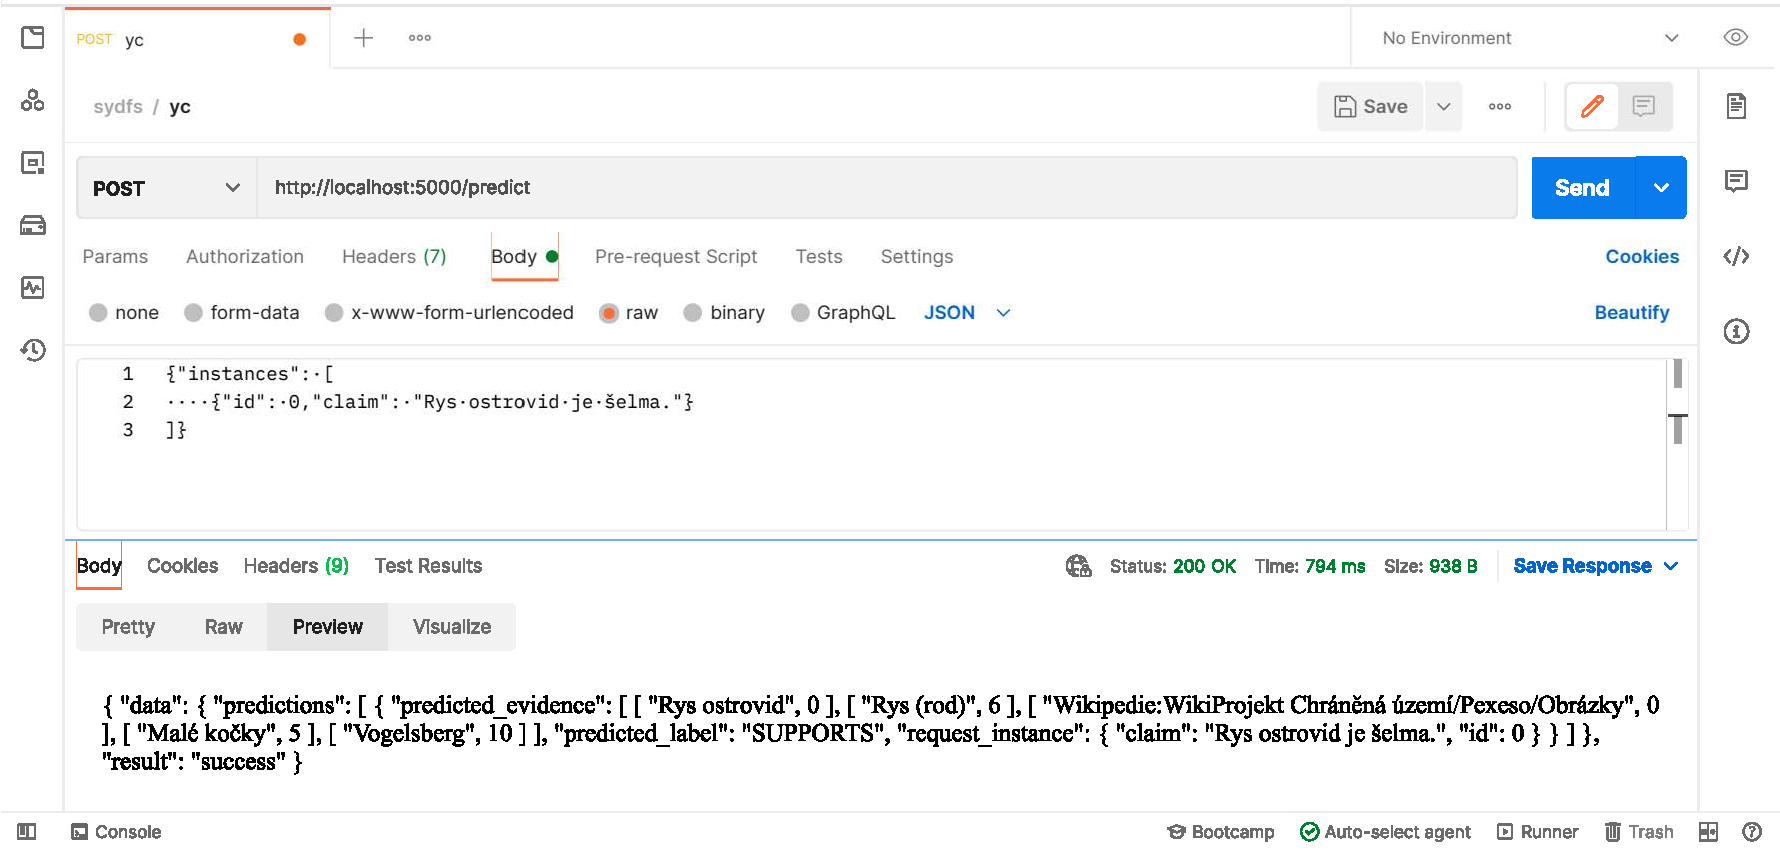
\includegraphics[width=18cm]{fig/rys.pdf}}}
\caption{Our \textsf{fever-cs-baseline} \textsf{API}, accessed through \textsf{Postman}}
\label{fig:rys}
\end{figure}
%--- /FIG

\subsection{Fact Search}


Through the course of the last year, our team supervisor Jan Drchal has produced a plethora of demonstrative production-like interfaces for our meetings with the \textsf{FSS} and \textsf{TAČR} stakeholders. The most notable interface is the \textsf{Fact Search} web console (Figure~\ref{fig:factsearch}) that emulates the outputs of the Document Retrieval task for an arbitrary claim, knowledge base and DR model.  

It computes the single-paragraph inference label using a legacy model for RTE (also known as NLI) for each retrieved document, to show the NLI use case. It also illustrates the Document Retrieval task referred to in~\ref{sec:document-retrieval} and gives a real-world example of an input data for our next chapter\dots

%--- FIG: UTF forms
\begin{figure}[H]
\vspace{2em}
\makebox[\textwidth][c]{\fcolorbox{ctublue}{white}{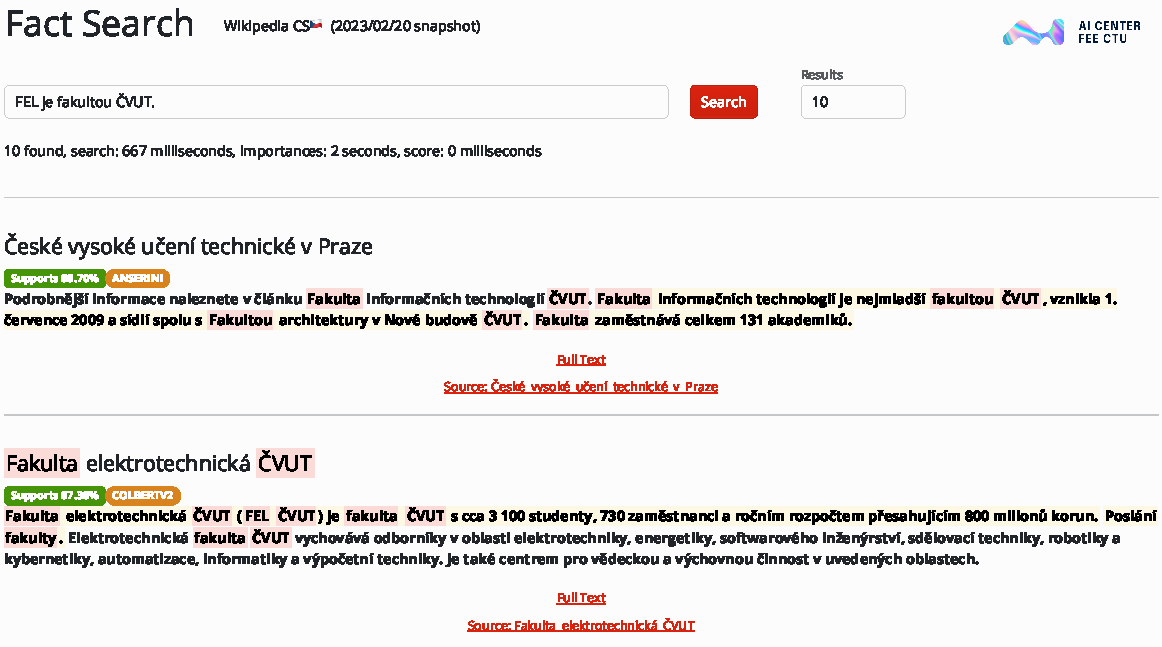
\includegraphics[width=17cm]{fig/factsearch.pdf}}}
\caption{\textsf{Fact Search} demo, authored by Jan Drchal, code at~\cite{honzagit}}
\label{fig:factsearch}
\end{figure}
%--- /FIG

%%!TEX ROOT=../ctutest.tex

\chapter{Natural Language Inference}
\label{chap:nli}

In chapter~\ref{chap:pipeline}, we have discussed the methods chosen by the \textsf{FCheck} team to retrieve a set of evidence relevant to the given claim. In the following chapter, we will proceed to show how to use these sets of evidence to infer whether the claim is provable or refutable.

This task is widely known as the \textit{Natural Language Inference} (NLI), previously known as the \textit{Recognizing Textual Entailment} (RTE). Whereas the RTE classification is bipartite (\textit{entailed}, \textit{no entailment}), the standard NLI classification is tripartite (\textit{entailed}, \textit{negation entailed}, \textit{no entailment})~\cite{overview}.

\section{Task definition}
\label{sec:task}
Given a textual claim $c_i$ and its set of evidence $E_{c_i}$ from the knowledge base, give a veracity label

$$h(c_i,E_{c_i}) = y$$

\noindent where $y\in\{\texttt{SUPPORTS},\texttt{REFUTES},\texttt{NOT ENOUGH INFO}\}$

\vspace{.3em}
For a practical instance, given a blinded datapoint formatted as in~\ref{list:fcheck-nli}, give the corresponding \texttt{label} given the \texttt{claim} and a \texttt{context}.

\section{Related work}
\label{sec:nlicorp}
We have examined the following NLI datasets in English, and their respective state-of-the-art classifiers, largerly based on transformer models resemblant to \textsf{BERT}~\cite{bert}
\begin{itemize}
    \item {\techbf Stanford NLI Corpus} ({\techbf SNLI})~\cite{snli:emnlp2015}: \"{A large annotated corpus for learning natural language inference} -- a long-term standard benchmark for the task of natural language inference. Corpus of \char`~570,000 human-written English sentence pairs manually labeled for balanced classification as \texttt{entailment}, \texttt{contradiction} or \texttt{neutral}.
    
    The state-of-the-art classifier as of May 2021 is \textsf{EFL}~\cite{wang2021entailment}, which reaches 93.1\% accuracy on the testing set. It uses a few-shot learning of \textsf{RoBERTa}~\cite{roberta} on the specific NLI classes.
    
    \item {\techbf Multi-Genre Natural Language Inference} ({\techbf MultiNLI})~\cite{multinli} was collected for the \textsf{RepEval} shared task. It is  modeled after \textsf{SNLI} and distributed in the same format. It contains \char`~433,000 sentence pairs and covers various genres of spoken and written English, such as \textsc{Fiction} extracted from project \textsf{Gutenberg}\footnote{\url{https://gutenberg.org}}, \textsc{Travel} from \textsf{Berlitz} travel guides, etc\dots
    
    As of May 2021, The highest accuracy (92.2\% in \textsc{Matched}, 91.7\% in \textsc{Mismatched}) was reached by \textsf{Google}'s \textsf{T5-11B}\footnote{Stands for a \textbf{T}ext-\textbf{t}o-\textbf{T}ext \textbf{T}ransfer \textbf{T}ransformer with \textbf{11 B}illions of parameters.}~\cite{t5-11b} through \textit{transfer learning}, i. e. fine-tuning a large model pretrained on a data-rich task to the specific downstream task of NLI.
    
    \item {\techbf Adversarial NLI} ({\techbf ANLI})~\cite{anli} - human-and-model-in-the-loop dataset, consisting of three rounds of increasing complexity and difficulty (\textsf{A1}, \textsf{A2}, \textsf{A3}), that include explanations provided by annotators. The total size of all sets is about 170K sentence pairs.
    
    The state-of-the-art solver \textsf{InfoBERT}~\cite{infobert} applies a further adversarial training to the \textsf{RoBERTa} model to achieve 75\% accuracy on the \textsf{A1} test set and 58.3\% overall, using all the samples of \textsf{A1}, \textsf{A2}, \textsf{A3} test sets combined.
    \item {\techbf FEVER for NLI} is a simple conversion of the \textsf{FEVER} dataset from its original format to the $(query,context)$ pairs, made as a byproduct of the UNC classifier~\cite{nie2019combining} from the \textsf{FEVER} shared task.
    
    This specific classifier was taught using NSMN\footnote{Neural Semantic Matching Network} augmented by a \"{relatedness} score and ontological knowledge from \textsf{WordNet}, and achieved  68.16\% label accuracy. 
\end{itemize}

\subsection{Slavonic Language Models}
As nearly every solution examined in the Section~\ref{sec:nlicorp} relies on the transfer learning, fine-tuning a large Transformer (\ref{sec:transformers}) language model to learn the predictions on a \textit{down-stream} task, let this be the strategy we employ for the preliminary entailment experiments as well.

First of all, let us examine the models that may already \"{speak} Czech: 
\begin{itemize} 
    \item {\techbf{Multilingual BERT}} ({\techbf mBERT}) -- is, basically, a variation of \textsf{Google}'s famed \textsf{BERT}$_\textsf{BASE}$ model~\cite{bert} for multiple languages, trained on the \textit{Masked Language Modeling} (\textit{MLM}) and \textit{Next Sentence Prediction} (\textit{NSP}) tasks using 104 localizations of \textsf{Wikipedia}. In our team, it has already been used for the \textit{knowledge scope} computations (\ref{sec:knowledge-scopes}), as well as for the Document Retrieval task by~\cite{rypar,michal} (\ref{tab:dr}) towards encouraging results
    
    \item {\techbf{SlavicBERT}}~\cite{slavicbert} -- similar to \textsf{mBERT}, trained on joint Bulgarian, Czech, Polish and Russian corpora
   
   \item {\techbf{HerBERT Ullrich}} -- haha, nothing here. Just testing your \textit{attention} (\ref{sec:transformers})\footnote{\textit{Ba dum tss.}}
   \item {\techbf XLM-RoBERTa}~\cite{xlm-roberta} is the crosslingual version of \textsf{RoBERTa}, trained solely on the \textit{MLM} task on a corpus significantly larger than of \textsf{Wikipedia} -- the cleaned \textsf{CommonCrawl} data it is trained on comes at 2.5TB of storage-size. As of May 2021, the \textsf{RoBERTa} derivates achieve the sota performance in many NLI benchmarks\footnote{See at \url{https://paperswithcode.com/task/natural-language-inference/latest}}
    \item {\techbf{CZERT}}~\cite{czert} is a recent arrival to the \textsf{BERT} family -- a couple of monolingual Czech models that are trained using 340K sentences from the Czech \textsf{Wikipedia}, \textsf{Czech National Corpus} and crawled Czech news. The models are based on \textsf{BERT} and \textsf{ALBERT}~\cite{albert} and are trained with random initialization on the \textit{MLM}+\textit{NSP} and \textit{MLM}+\textit{Sentence Order Prediction} tasks, respectively.
\end{itemize}
\section{Modified ČTK dataset}
\label{sec:modified-ctk}
On top of the \textsf{ČTK} dataset~(Section \ref{sec:dataset-latest}), we propose the following simple methods of augmentation for the NLI task, using the auxiliary data collected in Chapter~\ref{chap:collection}.

To emulate a set of evidence for the \texttt{NOT ENOUGH INFO} annotations in task~\ref{sec:task}, one can simply sample paragraphs from the knowledge scope of this claim. We propose to sample multiple different evidence sets for a single \texttt{NEI} claim in order to balance the dataset.

In~\ref{sub:conditional}, we have introduced the concept of \textit{conditional labeling}. In terms of natural language inference, the labels with nonempty \texttt{condition} can be included twice:

\begin{enumerate}
    \item As \texttt{NOT ENOUGH INFO} annotations
    \item As \texttt{SUPPORTS} or \texttt{REFUTES} annotations, if we consider larger evidence sets, augmented with the knowledge listed in \texttt{condition}
\end{enumerate}

This behaviours have been added to our dataset export \textsf{API} (\ref{sec:export}) using the \textsf{HTTP GET} activation parameters \texttt{simulateNei=1} and \texttt{condition=double}, respectively.

\section{NLI Experiments}

In the following section, we will conclude a set of preliminary Natural Language Inference experiments, largely relying on the \textsf{AIC FactCheck}'s internal set of modules for model training and evaluation by~\cite{honzagit}, that has shown promising preliminary results after the first wave of annotations. 

The \textsf{BERT}-like models are handled with ease using the \textsf{Huggingface} \texttt{transformers}~\cite{huggingface} and the \textsf{sBERT} \texttt{sentence\_transformers} \cite{sentence-transformers} libraries. We would like to thank the authors of all the aforementioned software for making it easy to obtain relevant results without having to delve too deep into the underlying compatibility challenges.

\subsection{Data Consistency Remarks}
As the experiments from this chapter were to be run simultaneously with the dataset collection and evaluation from the Chapters~\ref{chap:ctk}  and~\ref{chap:dataset}, naturally, we have run into a \textit{race condition}. That is, at a certain point we had to fix a single legacy dataset version to be used for all further runs of our experiments and to proceed with the production dataset refinement in separation from the NLI application. 

The dataset we fixed for this task is the \textsf{ČTK v2 CSV} (\ref{item:ctk-csv}) exported in early May 2021, that does not yet include all the refinements described in Chapter~\ref{chap:dataset}. However, it features all the datapoints from the first three waves, similarly to \textsf{ČTK v2.1}. For the completeness, we attach the \textsf{JSONL} reprint of the data in our dataset cloud storage\footnote{\url{http://bertik.net/ctk}}, even though in practice it is being generated on-demand from the \textsf{CSV db} dump using a fixed\textit{ seed of randomness}. 

As we will be using the \textit{stratified} split of our dataset, de facto disabling the \textit{accuracy} metric, we will be comparing our models based on their the $F$-score, which is a standard benchmark for the NLI task~\cite{poliak}.

\subsection{Experiments on Sentence\_transformers Models}
\label{sec:expts}
Using a set of ad--hoc \textsf{Jupyter} notebooks\footnote{\url{https://gitlab.fel.cvut.cz/factchecking/nli}} powered by the \textsf{sentence\_transformers} and the shared codebase of the \textsf{AIC/FactCheck} team, we have downloaded the pretrained \textsf{SlavicBERT} and \textsf{mBERT} models in their \textit{cased} defaults, provided by the \textsf{DeepPavlov}~\cite{deeppavlov}. Furthermore, we have acquired an \textsf{XLM-RoBERTa} model, fine-tuned on an NLI-related \textit{SQuAD2}~\cite{squad} \textit{down-stream task}. This model was provided by \textsf{deepset}~\cite{deepset}.



Starting from these three base models, we have initiated a series of model training tasks on the \textsf{RCI Cluster}, varying in the batch size and the overall number of epochs. The latter was typically not of an overwhelming significance, as, given the relatively small \textsf{train} split of the \textsf{ČTK} dataset, models soon started to overfit -- see Figure~\ref{tab:overfitting}. In such cases, we kept the \textsf{dev}-optimal model, tossing the later epochs.

%%%%

\begin{table}[H]
\begin{ctucolortab}
\begin{tabular}{|c|c|c|}
\hline
\textbf{epoch} & \textbf{\textsf{train} acc. }   &\textbf{ \textsf{dev} acc.}    \\
\hline
0.     & 0.80 & 0.77  \\
1.     & 0.93 & \textbf{0.87}  \\
2.     & 0.96 & 0.81  \\
3.     & 0.98 & 0.85 \\
4.     & 0.98 & 0.84 \\
 \vdots      & \vdots   &  \vdots \\
100.   & \textbf{1.00}  & 0.81 \\  
\hline
\end{tabular}
\end{ctucolortab}
\caption{The progress of \textsf{XLM-RoBERTa@SQuAD2\_bs4} in the \textsf{train} and \textsf{dev} accuracies during 100 epochs of training on the \textsf{ČTK} dataset}
    \label{tab:overfitting}
\end{table} % Overfit

Despite that, we have set a strong baseline for the future NLI experiments on the \textsf{ČTK} datasets with our \textsf{XLM-RoBERTa} model scoring an $F$-value of \textbf{0.86}. For reference, the \cite{fever} baseline scored 80.82\% \textit{accuracy} in a similar setting (\textit{NearestP} -- nearest page for a \textsf{NEI} context) on \textsf{Wikipedia}, using a Decomposable Attention model.

\begin{table}[H]
    \centering
    \makebox[\textwidth][c]{\begin{ctucolortab}
    \begin{tabular}{|lr|rr|rr|}
    \hline
    \textbf{\textsf{ČTK v2 CSV} split:}&&\multicolumn{2}{c|}{\textsf{test}}&\multicolumn{2}{c|}{\textsf{dev}}\\
    \hline
    \textbf{model}&\footnotesize{$|batch|$}& \textbf{\footnotesize{micro-}$F_1$}&\textbf{\footnotesize{macro-}$F_1$} &\textbf{\footnotesize{micro-}$F_1$}&\textbf{\footnotesize{macro-}$F_1$}\\
    \hline
        \textsf{SlavicBERT} &2 &\textit{0.743}&0.700&0.771&0.735\\
        \textsf{SlavicBERT} &5 &\textit{0.741}&0.702&0.782&0.757\\
        \textsf{mBERT} &3 &\textit{0.727}&0.686&0.710&0.667\\
        \textsf{mBERT} &10 &\textit{0.743}&0.717&0.742&0.721\\
        \textsf{XLM-RoBERTa @ SQuAD2} &2 &\textit{0.807}&0.769&0.842&0.815\\
        \textbf{\textsf{XLM-RoBERTa @ SQuAD2}} &\textbf{4} &\textbf{\textit{0.855}}&\textbf{0.840}&\textbf{0.866}&\textbf{0.849}\\
        \textsf{XLM-RoBERTa @ SQuAD2} &7 &\textit{0.835}&0.819&0.851&0.838\\
        \hline
    \end{tabular}
    \end{ctucolortab}}
    \caption[$F$-score comparison of our \textsf{BERT}-like NLI models]{$F$-score (\textbf{micro-$F_1$}) comparison of our \textsf{BERT}-like models for the \textit{NLI} task on the {\techbf ČTK} data, experimenting with different training \textit{batch sizes}. \textit{Coursive} decisive, \textbf{bold} best.}
    \label{tab:nli}
\end{table} % f1
%%%

Furthermore, we render the confusion matrices for two of our strongest models -- the \textsf{XLM-RoBERTa} and the \textsf{SlavicBERT}, to see the distribution of their \textsf{test}-set \textit{(mis-)classifications} -- we see that the main disadvantage of \textsf{SlavicBERT} compared to the stronger \textsf{XLM-RoBERTa} is the understanding of the \texttt{REFUTES} annotations.
%--- FIG: UTF forms
\begin{figure}[H]
\vspace{2em}
\makebox[\textwidth][c]{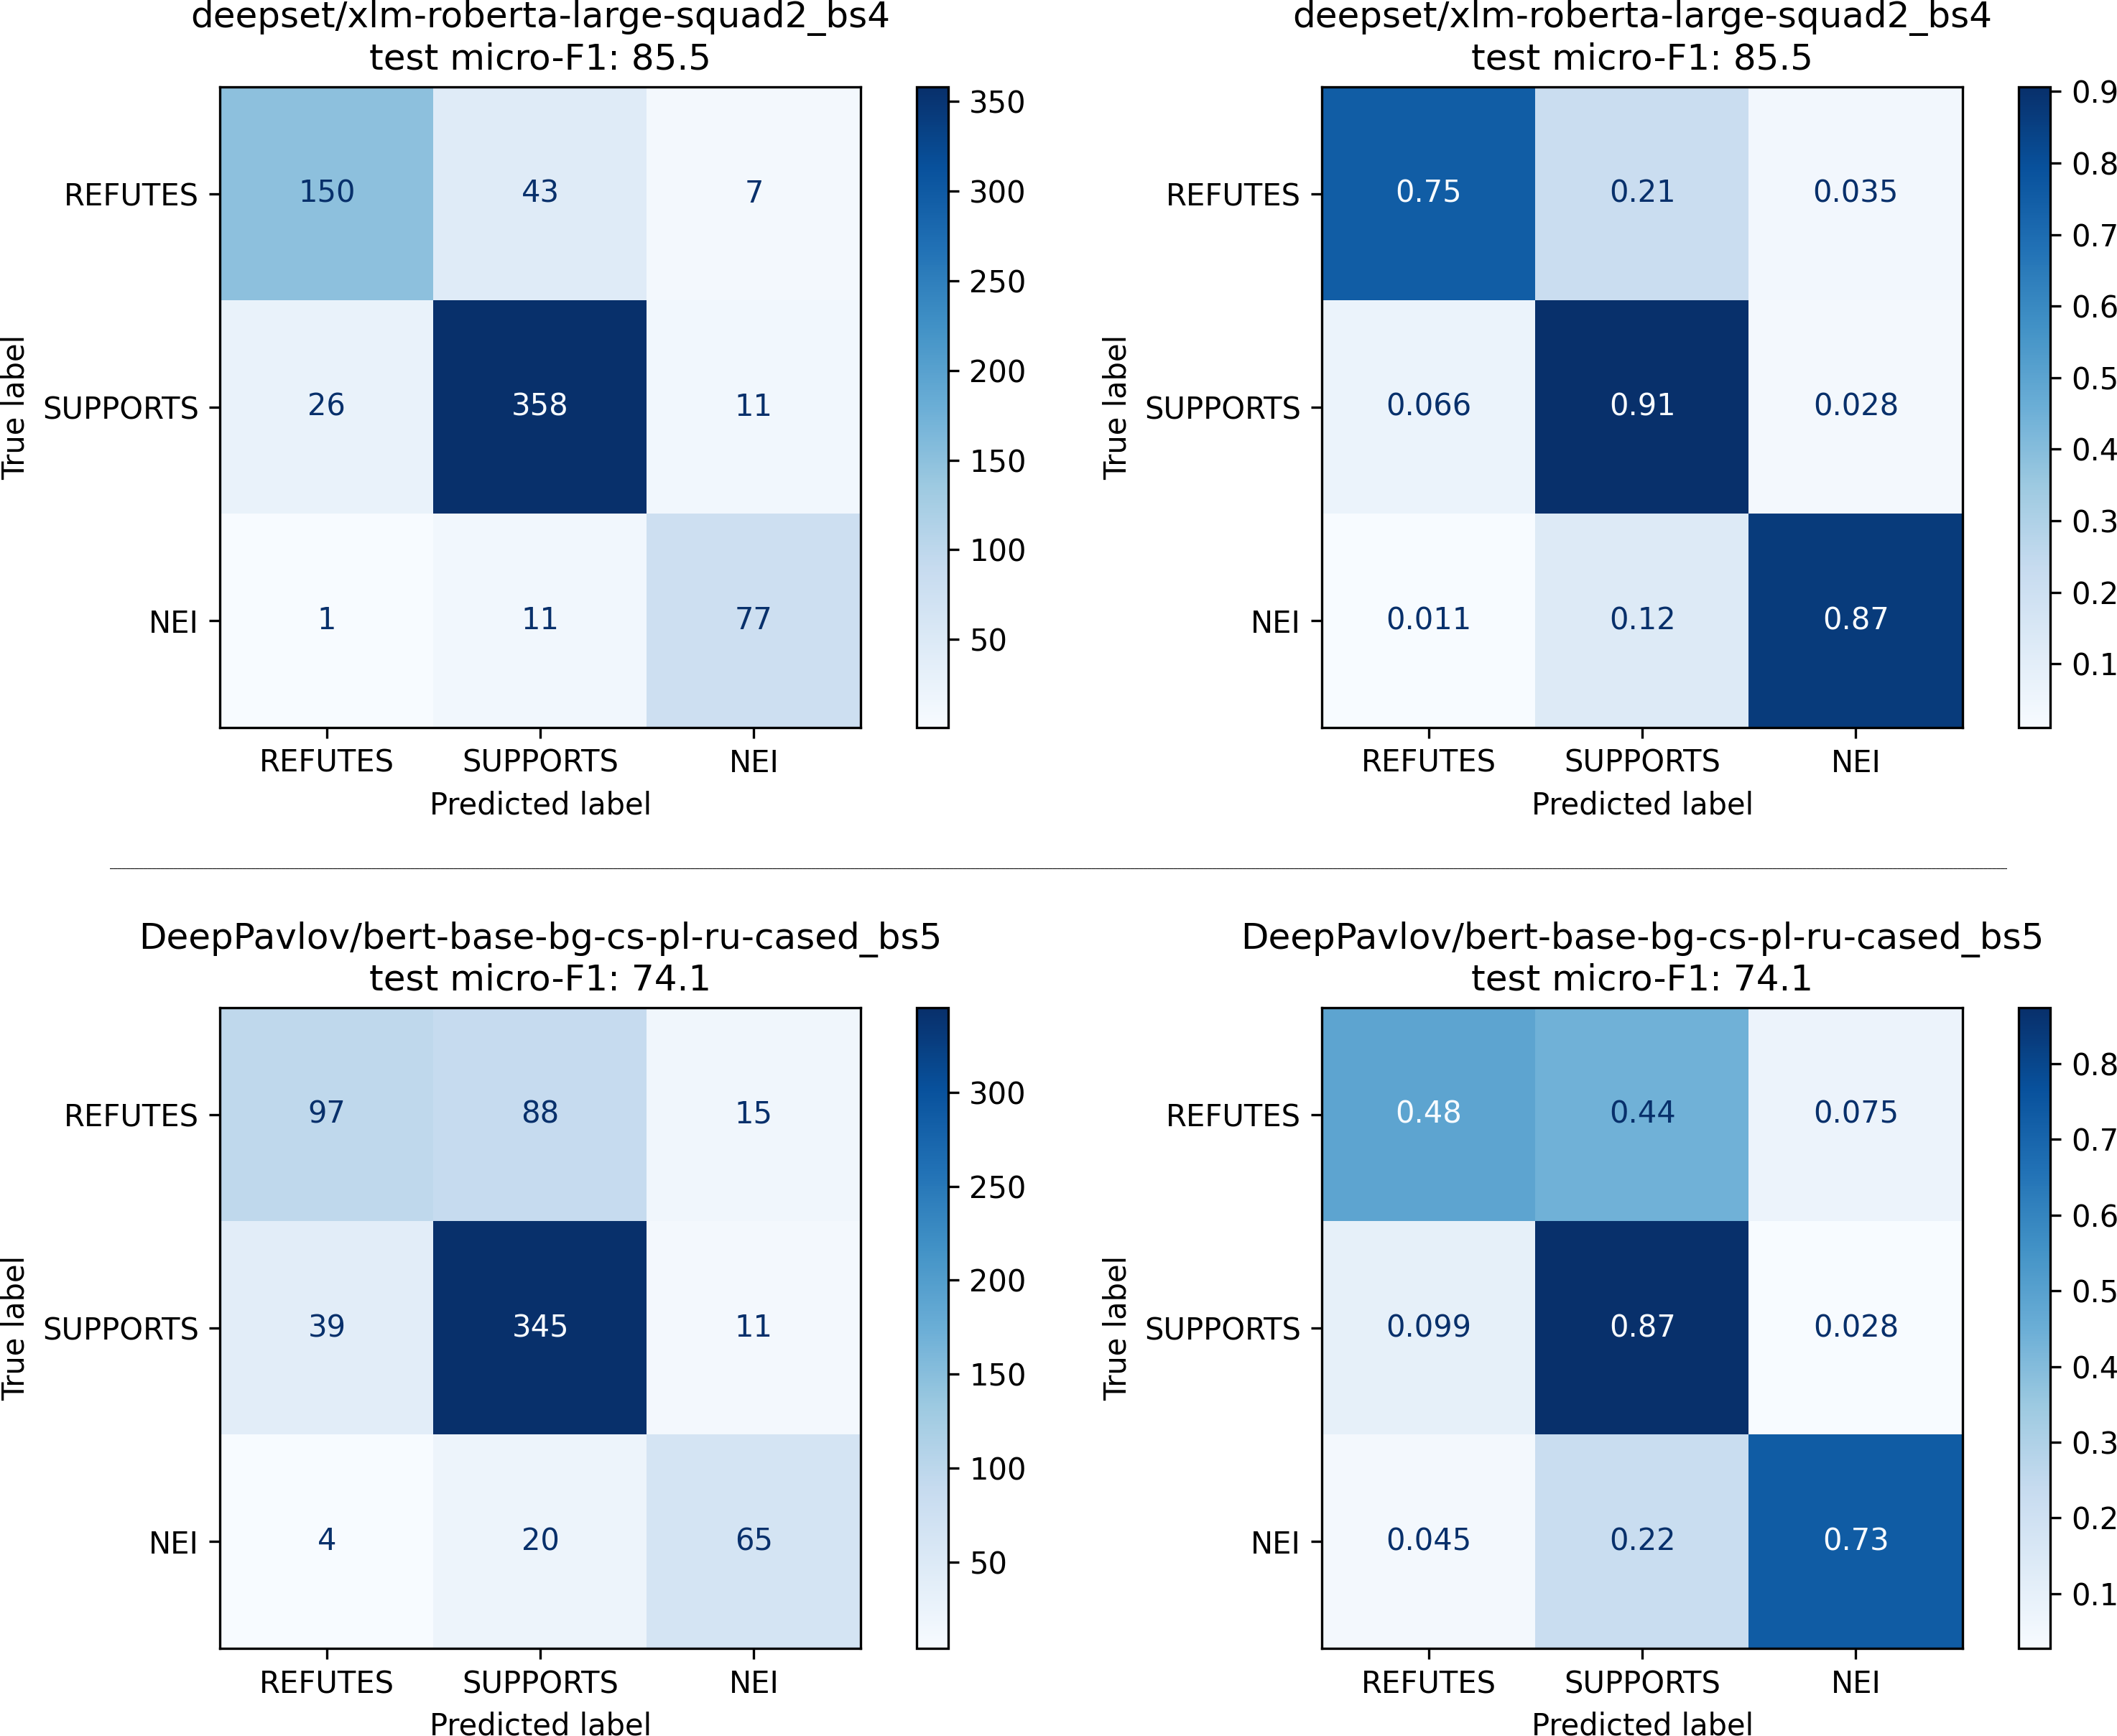
\includegraphics[width=17cm]{fig/confmat.png}}
\caption[Confusion Matrices of XLM-RoBERTa and SlavicBERT]{The confusion matrices of \textsf{XLM-RoBERTa} finetuned on \textit{SQuAD2} and the \textsf{SlavicBert} models for Natural Language Inference on \textsf{ČTK} test data}
\label{fig:confmat}
\end{figure} %confmatky
%--- /FIG



\subsection{Machine-translated NLI corpora}
To address the \textit{overfitting} (Table~\ref{tab:overfitting}) issue in our future experiments, our team at \textsf{AIC} has internally obtained a machine-translated Czech localization for each of the corpora listed in~\ref{sec:nlicorp},  using the \textsf{Google Translate API}. The scheme is simpler than that from~\ref{sec:fevercs}, as their formats are closely resemblant to the \texttt{nli} \textsf{FCheck} export (Figure~\ref{list:fcheck-nli}), i.e., a set of plain text pairs and their labels.

In future, the Czech \textsf{SNLI}, \textsf{MultiNLI}, \textsf{ANLI} or \textsf{FEVERNLI} datasets could be either used directly to augment the \textsf{ČTK NLI train} dataset, or to construct a \textit{down-stream task} for NLI in Czech.

In the weeks subsequent to the submission of this thesis, we will examine the licensing of the aforementioned corpora, and, if allowed, publish their Czech localizations in a cloud storage\footnote{\texttt{http://bertik.net/nli\_corpora}} to supplement this thesis.


\section{Experiments Wrapup}
In our last full chapter, we have used the data collected during our annotation experiments in Chapter~\ref{chap:ctk} to train a round of Czech Natural Language Inference classifiers. The strongest of them, \textsf{XLM-RoBERTa} sets a vital benchmark for its future successors, and is ready to be experimentally used in the production environment, provided there is a reliable \textit{Document Retriever} to feed its input (Figure~\ref{fig:pipeline}).

We attach the experimental notebooks\footnote{\url{https://gitlab.fel.cvut.cz/factchecking/nli}} used to train and validate our models, as well as the resulting model\footnote{\url{http://bertik.net/ctk-xlm-roberta}} in a hope for reproducibility of our experiments, however, the code quality is incomparable with the PHP application from Chapter~\ref{chap:ctk}.

% say that it is analogous to RTE
% NLI Experiments
%%!TEX ROOT=../ctutest.tex

\chapter{Conclusion}
\label{chap:conclusion}
\label{chap:proposed}
Our work has addressed the lack of a fact-verification dataset in Czech in two ways:

Firstly, it established a scheme of transferring an English \textsf{ENWiki}-corpus-based \textsf{FEVER} dataset to the Czech language using Machine Translation and the cross-lingual mapping of \textsf{WikiMedia API}, obtaining a set of a total of 127K translated claims along with their veracity labels and evidence within the \textsf{CSWiki} corpus, which we call the \textsf{FEVER CS} dataset.

Secondly, we prepared a series of human-annotation experiments, that were conducted with 163 annotators, utilizing the collaboration with the \textsf{Faculty of Social Sciences of Charles University} towards collecting about 10K \db{Claim} and \db{Label} data points stemming from our application-specific \textsf{ČTK Archive} knowledge base, achieving an inter-annotator aggreement of 0.63, measured using the 4-way Fleiss' $\kappa$.

For the annotations, we have built a novel annotation platform from the ground up, naming it the \textsf{FCheck Annotations Platform} and publishing it as an open-source project. Subsequently, we have used our platform to export the novel \textsf{ČTK} dataset, that contains 3,295 textual claims along with their veracity labeling and \textsf{ČTK}-based sets of conclusive evidence, extracted from the results earlier annotation experiments.

Finally, we deem this dataset eligible for training statistical models for the task of Natural Language Inference, demonstrating the usage of our data on transfer-learning a triple of Transformer networks -- \textsf{XLM-RoBERTa}, \textsf{SlavicBERT} and \textsf{multilingualBERT}, the first of which scores \textbf{85.5\%} micro-$F_1$ on the \textsf{ČTK} claim veracity labeling task.

\section{Proposed solutions}
At the end of every chapter, we provide a textual \textit{wrapup} of its result, along with remarks on its reproducibility, and, where possible, a ready-made solution in form of an open-source code, or prebuilt models and datasets shared through a public cloud-storage link.

This is to encourage any future research on the topic, as well as to challenge our results and their credibility.

\section{Future research goals}
Our work at \textsf{AIC FactCheck} is far from over. After the publication of the \textsf{ČTK} dataset and the baseline NLI classifier, we are about to pursue some of the following goals that arised from the findings in previous chapters:

\begin{enumerate}
    \item The solution for the \textit{overfitting} issue from Chapter 7 should be examined, using some of the attached localized \textsf{SNLI},  \textsf{MultiNLI},  \textsf{ANLI}  and \textsf{FEVER-NLI} sets, as outlined in the previous Chapter \textit{wrapup}
    \item The novel monolingual Czech \textbf{\textsf{CZERT}} model is to be trained and examined on the same tasks as the other models from the Chapter 7
    \item \textbf{\textsf{The FEVER CS Baseline}} end-to-end containerized pipeline should be updated with our resulting models and that of~\cite{rypar} for the production purposes
    \item The set of \tdvab{} \textbf{\textsf{Claim Mutations}} (Figure~\ref{fig:mutations}) collected by the \textsf{FCheck} platform is to be examined and challenged with the dataset balance in mind, as the same set of mutation tasks yielded a significantly label-unbalanced dataset to \textit{us} (Chapter~\ref{chap:dataset}), to~\cite{fever} and to~\cite{danish}, all of them in favour of the \texttt{SUPPORTS annotation}
\end{enumerate}

% future challenges

%\bibliographystyle{amsalpha}
\bibliographystyle{apalike}
\bibliography{minimum}
\appendix
%\chapter{Czech-English data translations}
\section{Translated figures}

\begin{figure}[H]
\centering
 \fbox{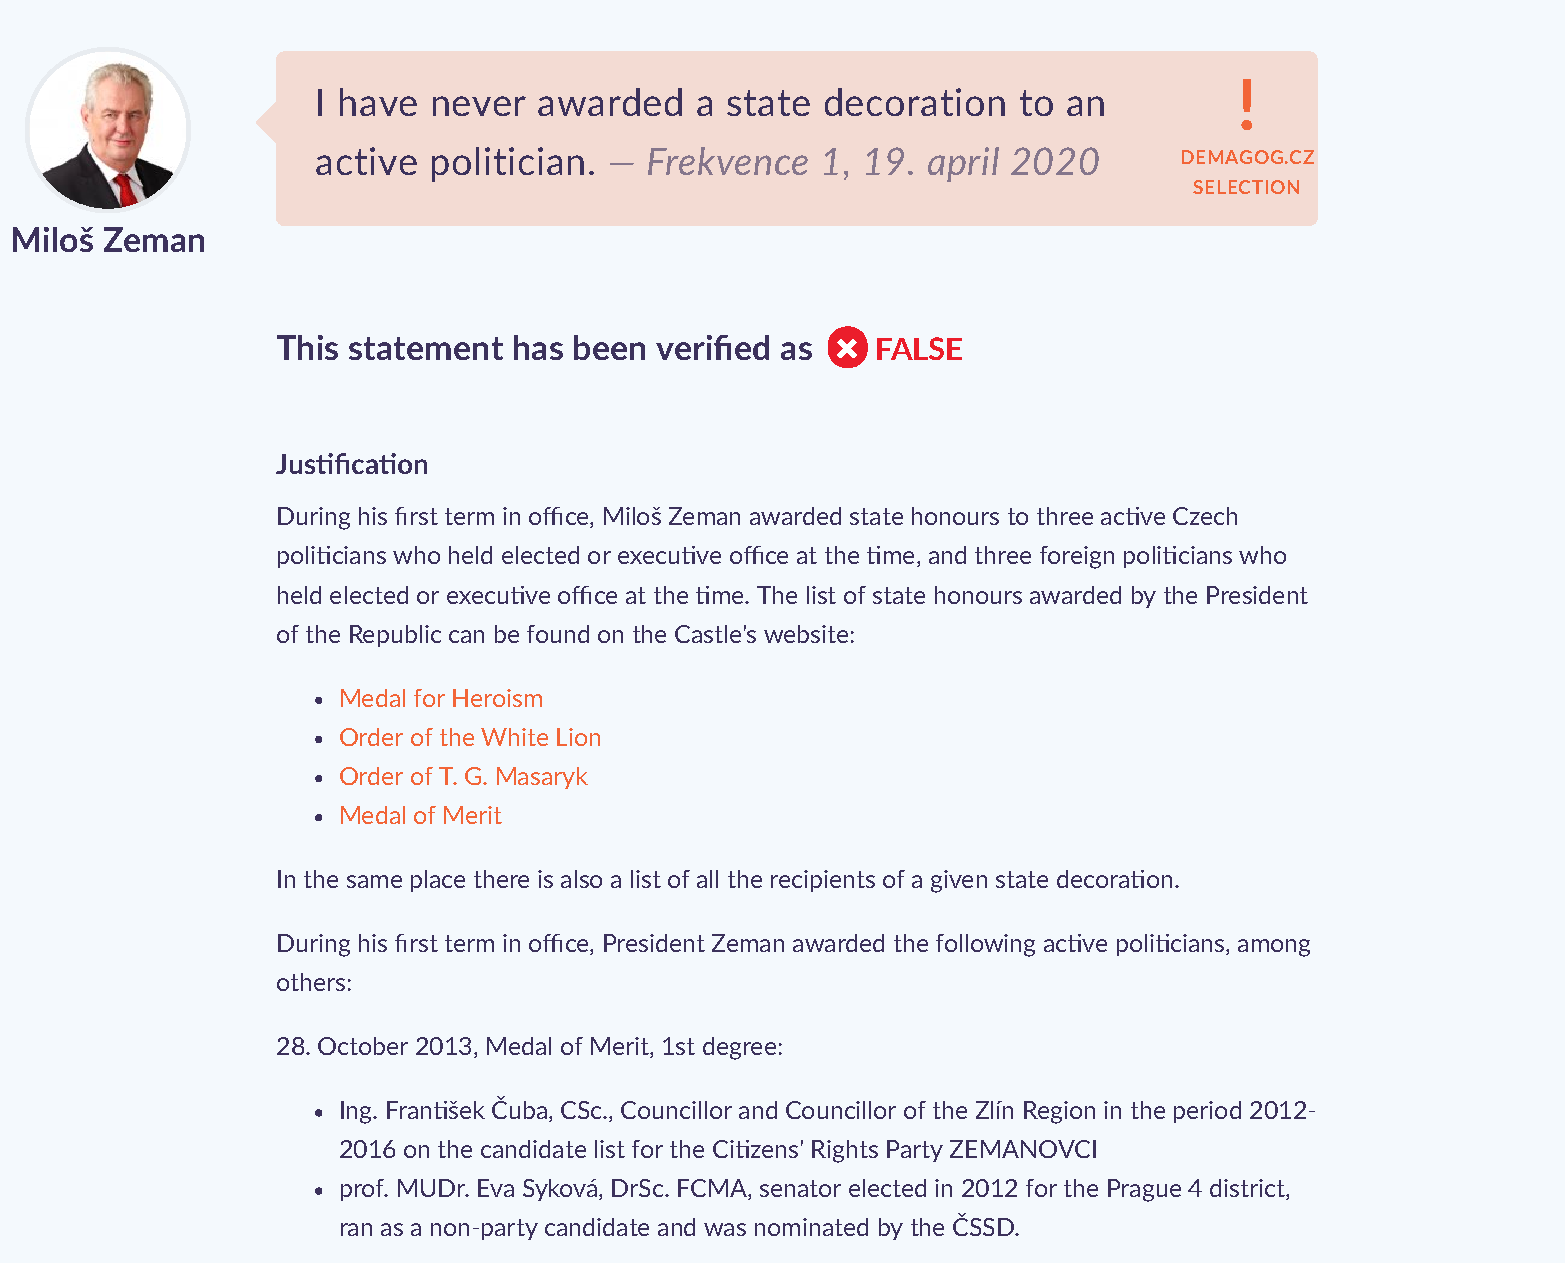
\includegraphics[width=\textwidth]{fig/demagog_en.pdf}}
\caption[English Translation of Figure~\ref{fig:demagog}]{Translated fact verification from Czech portal \textsf{Demagog.cz} -- original in Figure~\ref{fig:demagog}}
\label{trans:demagog}
\end{figure}

\begin{figure}
\thisfloatpagestyle{empty}
\vspace{-2cm}
 \makebox[\textwidth][c]{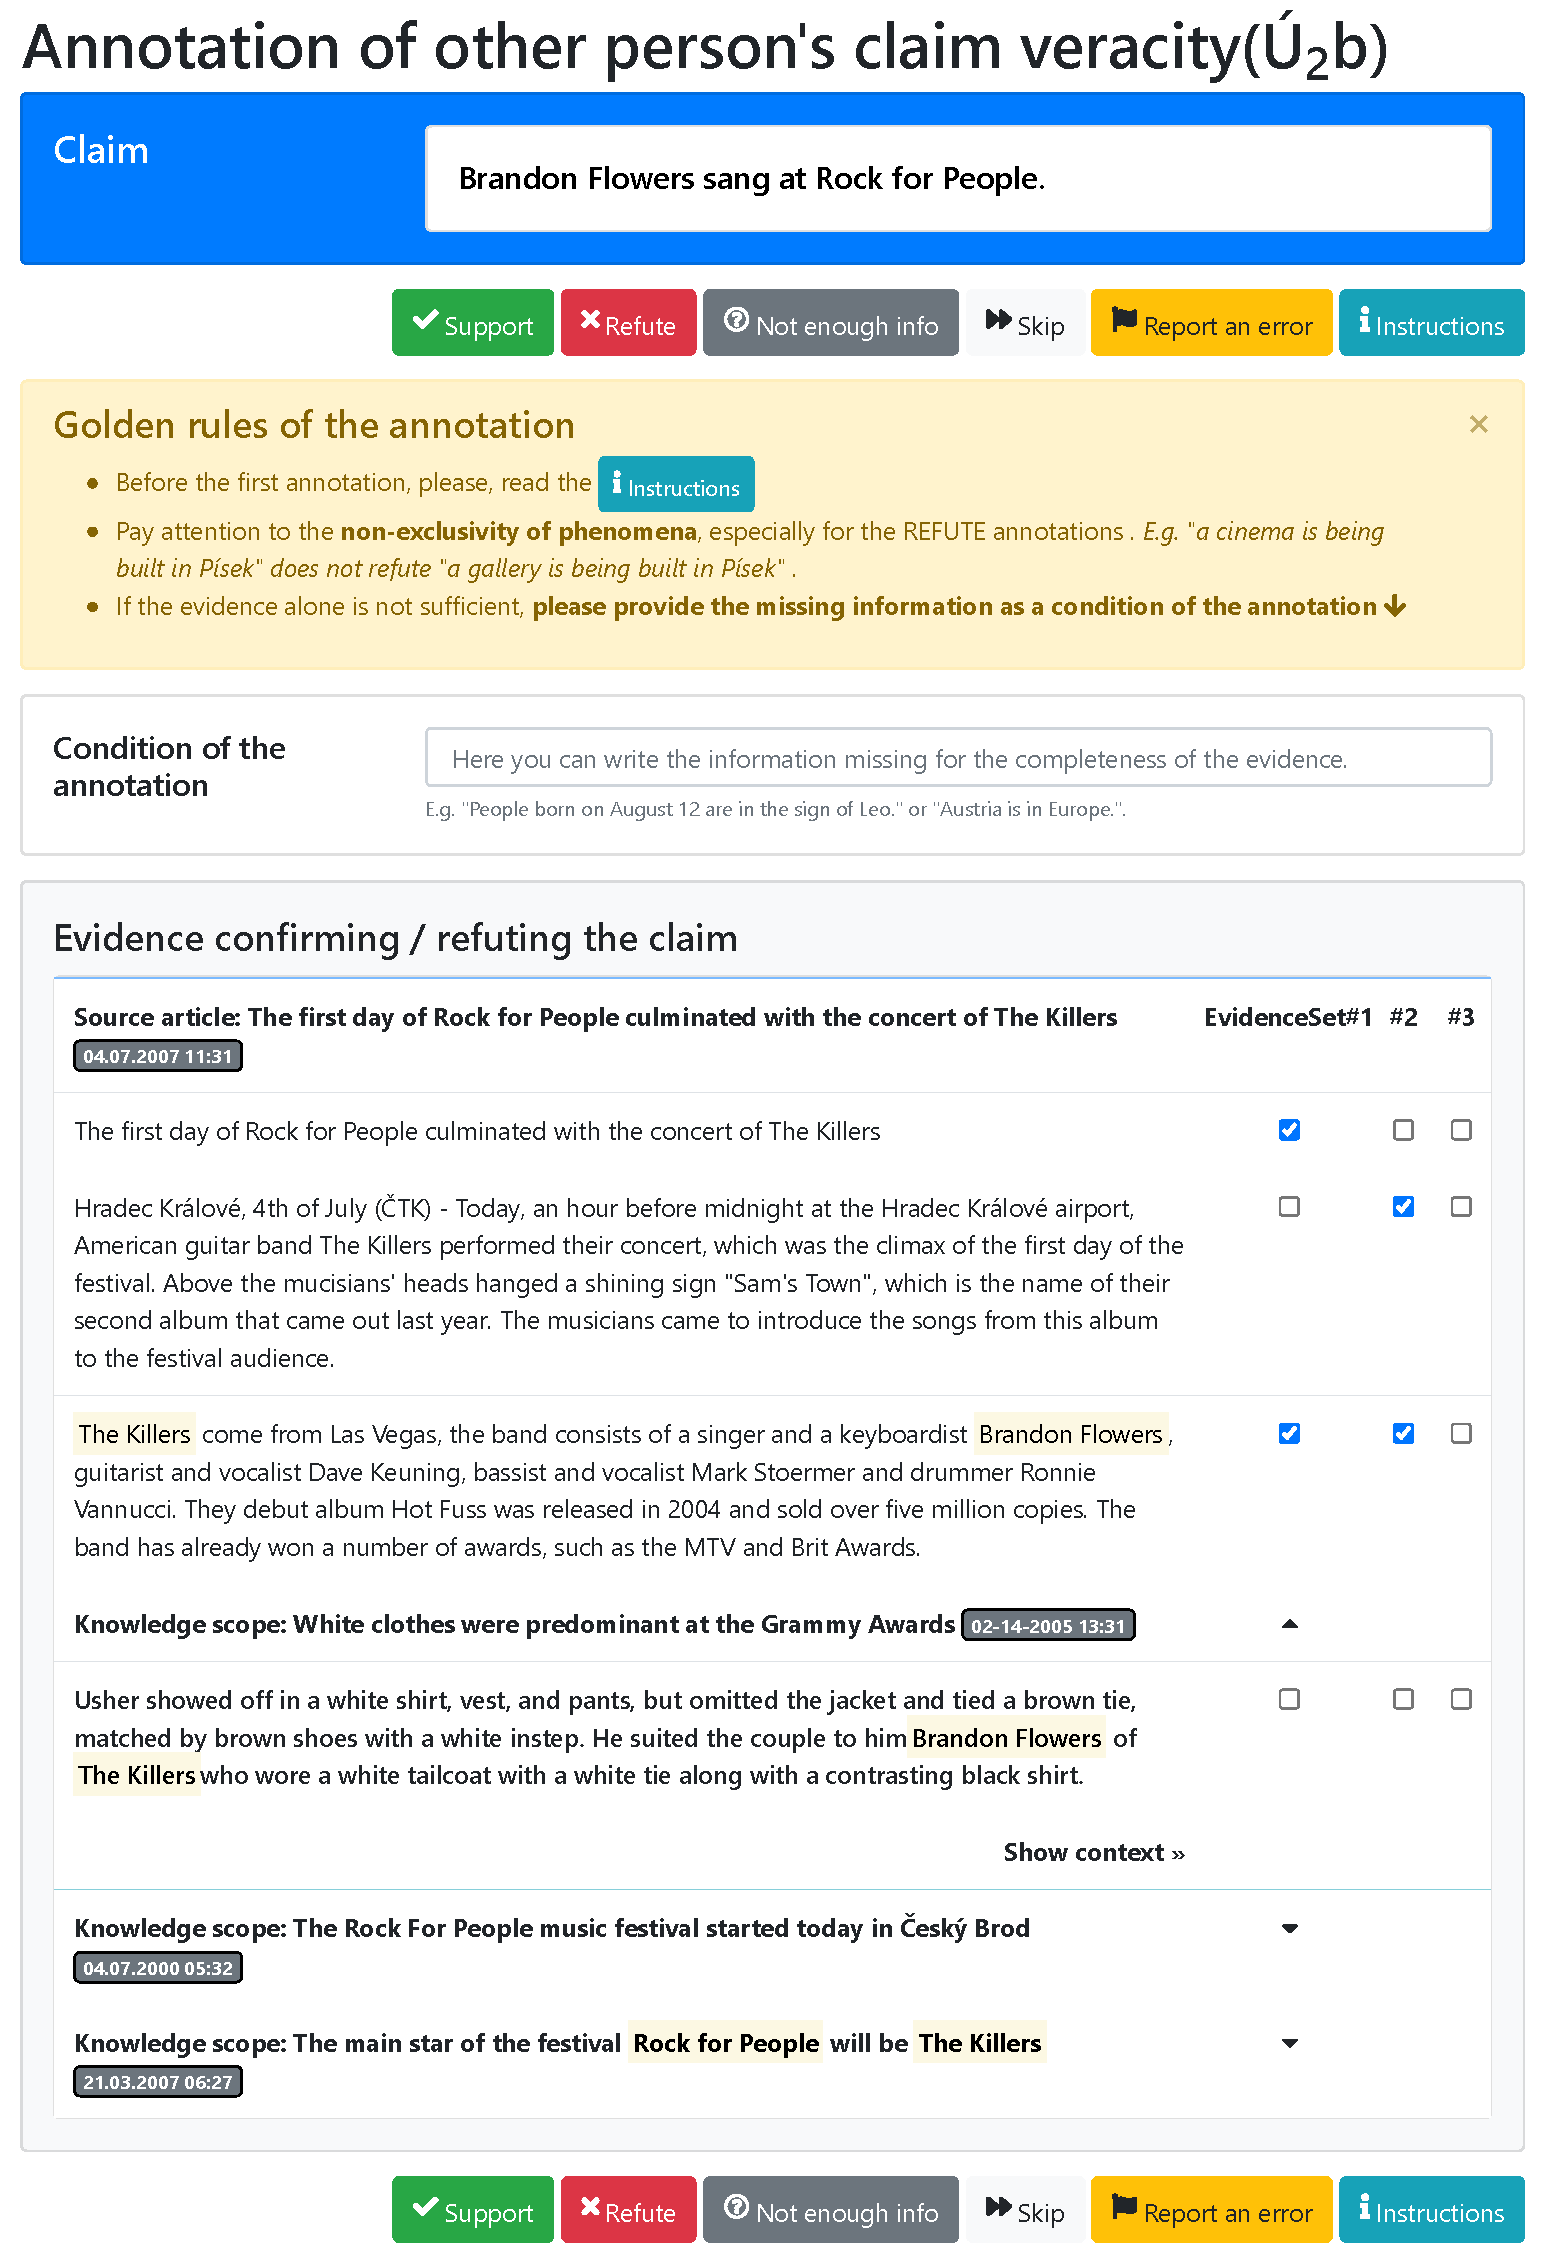
\includegraphics[width=18cm]{fig/annotation_en.pdf}}
\caption[English Translation of Figure~\ref{fig:annotation}]{The labelling interface of \textsf{FCheck} platform. Czech original in Figure~\ref{fig:annotation}}
\label{trans:annotation}
\end{figure}

\chapter{Acronyms}
\begin{description}
\item[BERT] Bidirectional Encoder Representations from Transformers
\item[FEVER] Fact Extraction and Verification -- series of Shared tasks focused on fact-checking
\item[CLI] Command-Line Interface
\item[NLI] Natural Language Inference
\item[ČTK] Czech Press Agency
\end{description}


\end{document}